% -*- coding: utf-8 -*-
\documentclass[twocolumn]{article}
\usepackage{listings}
\usepackage{ctex}
\usepackage{graphicx}
\usepackage[a4paper, body={18cm,22cm}]{geometry}
\usepackage{amsmath,amssymb,amstext,wasysym,enumerate,graphicx,physics,extarrows}
\usepackage{float,abstract,indentfirst}
\usepackage{array}
\usepackage{booktabs}
\usepackage{multirow}
\usepackage{url}
\usepackage{diagbox}
\renewcommand\arraystretch{1.4}
\usepackage{indentfirst}
\setlength{\parindent}{2em}
\usepackage{tcolorbox}
\tcbuselibrary{most}
\usepackage{tikz}
\usetikzlibrary{positioning}


\usepackage[breaklinks,colorlinks,linkcolor=black,citecolor=black,urlcolor=black]{hyperref}

\usepackage{listings}
\usepackage{xcolor}
\lstset{
	numbers=left, 
	numberstyle= \tiny, 
	keywordstyle= \color{ blue!70},
	commentstyle= \color{red!50!green!50!blue!50}, 
	frame=shadowbox, % 阴影效果
	rulesepcolor= \color{ red!20!green!20!blue!20} ,
	escapeinside=``, % 英文分号中可写入中文
	xleftmargin=2em,xrightmargin=2em, aboveskip=1em,
	basicstyle=\footnotesize,
	framexleftmargin=2em
} 


\geometry{left=2.8cm,right=2.2cm,top=2.5cm,bottom=2.5cm}

\graphicspath{{figures/}}

\newtcolorbox{cbox}[2][gray]{colback=#1!5!white,
	colframe=#1!75!black,fonttitle=\bfseries,
	title={#2},
	sharp corners}

\newtcolorbox{cnote}[1][gray]{blanker,boxsep=5pt,sharp corners,
	borderline west={2pt}{0pt}{#1} }

\newtcbox{\cboxone}[2][gray]{colback=#1!5!white,
	colframe=#1!75!black,fonttitle=\bfseries,
	title={#2},
	sharp corners}

\newtcbox{\cword}[1][green]{on line,
	arc=0pt,outer arc=0pt,colback=#1!10!white,colframe=#1!50!black,
	boxsep=0pt,left=1pt,right=1pt,top=1pt,bottom=1pt,
	boxrule=0pt,bottomrule=1pt,toprule=1pt}


\tikzset{global scale/.style={
		scale=#1,
		every node/.append style={scale=#1}
	}
}

\newcommand{\ii}{\mathrm{i}}
\newcommand{\ee}{\mathrm{e}}

\makeatletter
\newcommand{\rmnum}[1]{\romannumeral #1}
\newcommand{\Rmnum}[1]{\expandafter\@slowromancap\romannumeral #1@}
\makeatother


\begin{document}
	% By Lost@2021
	
	\begin{center}
		{\LARGE \heiti 宇宙学}\\
	\end{center}
	
	\section{引言}
	\par 
宇宙学是以宇宙为研究对象的一门学科。
\par 
宇宙:“上下四方曰宇,往古来今曰宙。”——战国·尸佼
\par 
宇宙是整个时空以及它的内容,包括一切天体等物质、能量。——Wikipedia

\subsection{宇宙学研究内容}
\begin{itemize}
	\item[1] 时间与空间
		\begin{itemize}
			\item[·] 几何结构:平直or弯曲?无限or有限?
			\item[·] 宇宙静态or演化 \quad 演化过程
		\end{itemize}
	\item[2] 宇宙介质
		\begin{itemize}
			\item[·] 物质
				\begin{itemize}
					\item[·] 可见:光子、重子物质
					\item[·] 不可见:暗物质,间接方法推知存在
				\end{itemize}
			\item[·] 这些物质占整个宇宙的比例?如何影响宇宙演化?
			\item[·] 暗能量:如何发现?所占比例?如何影响宇宙演化?
			\item[·] 物质、能量占比是否随时间演化,空间中如何分布?
			\item[·] 宇宙的物质形式是否变化?恒星与星系如何形成?
		\end{itemize}
\end{itemize}

\subsection{宇宙学的特殊性}
\begin{itemize}
	\item[1] 特殊性
	\begin{itemize}
		\item[1)] 研究对象:宇宙,仅此一个,只能靠观测和计算机模拟
		\item[2)] 我们在宇宙中的位置固定
			\begin{cbox}{在哪看有什么区别?}
				光传播速度有限$\Rightarrow$视界\quad 可观测宇宙
			\end{cbox}
		\item[3)] 宇宙演化过程复杂,牵涉知识广 
		\begin{itemize}
			\item[·] 时空演化——广义相对论GR
			\item[·] 高能粒子作用(早期)——粒子与核物理、统计力学
		\end{itemize}
	\end{itemize}
	\item[2] 和天体物理、天文学关系
	\par 天文学:
	\begin{itemize}
		\item[·] 宇宙学——研究整个宇宙的行为
		\item[·] 天体物理——研究单个或少量天体、星系
	\end{itemize}
\end{itemize}

\subsection{物理宇宙学简史}
\subsubsection{阶段一(1915-1930)}
\par 
初期,健康发展,在观测方面:
\begin{itemize}
	\item 1915 Einstein GR
	\item 1917 Einstein提出第一个物理宇宙学模型(Einstein模型)
	两条假设:
	\begin{itemize}
		\item[1)] 宇宙看作充满全空间的均匀介质
		\item[2)] 宇宙整体上看来静态,引入宇宙学常数$\Lambda$
	\end{itemize}
	\item 1920初 \quad 天文学家发现宇宙膨胀,抛弃了静态模型
	\item 1923 Slipher测量十多个漩涡星云,首次发现光谱大部分有红移现象,由Doppler效应,说明星云远离\\ 同一时期,Hubble发现星云实际是河外星系,人们意识到宇宙是以星系“分子”组成的气体
	
	\item 1929 Hubble定律,星系退行速度与距离成正比
	\begin{cnote}
		Hubble定律不仅说明宇宙在膨胀而且是以保持宇宙均匀性的方式膨胀,方式唯一
	\end{cnote}

\end{itemize}
\par 
在理论方面:
\begin{itemize}
	\item 1923 Friedmann采用不含宇宙学常数的模型,发现宇宙在引力作用下可以膨胀,预言了Hubble定律
\end{itemize}

\subsubsection{阶段二(1930-1960s)}
\par
挫折期,挫折原因:
\begin{itemize}
	\item[1] Hubble定律$v = H_0 d, H_0 = 500 \mathrm{km/s/Mpc}$得$\frac{1}{H_0}\sim \text{宇宙年龄} \sim \text{20亿年}$ \\
	Friedmann模型的理论基础:均匀性宇宙和宇宙演化服从GR
	\item[2] 反推宇宙有初始时刻$\rightarrow$宇宙创生,科学向宗教靠拢
\end{itemize}
\begin{cnote}
	Hubble定律是唯一能够达到宇宙均匀性的膨胀方式
\end{cnote}
\begin{itemize}
	\item 1940s Gamov提出宇宙演化论,观点:一切物质形态都不是亘古不变的
	\item 1950s 理论预言10K左右背景光谱
	\item 1950s中后期 $H_0 \sim 50-100 \mathrm{km/s/Mpc}$,解决了宇宙年龄矛盾
	\item 1965 宇宙微波背景辐射(CMB)发现$\Rightarrow$重新重视Hubble-Friedmann-Gamov宇宙理论
\end{itemize}

\subsubsection{阶段三(1970-now)}
\par 
蓬勃发展,发现:
\begin{itemize}
	\item[1] 微波背景的各向异性
	\item[2] 宇宙加速膨胀 $\rightarrow$ 暗能量(1998年)
	\item[3] 引力波的发现
	\item[4] 暗物质的发现
	\item[5] 暴涨理论的提出
\end{itemize}

	\section{观测概述}
	\subsection{黑夜为什么是黑的?Olbers佯谬}
\begin{itemize}
	\item 矛盾表述:
	$r$\textasciitilde$r + \dd r$球壳内恒星密度$n = \mathrm{const}$,恒星个数$N = 4 \pi r^2 n \dd r$,单颗恒星亮度$\frac{L}{4 \pi r^2}$,则球壳内总亮度$\frac{L}{4 \pi r^2} N = L n \dd r$,与距离无关 $\rightarrow$ 积分发散说明无黑夜,矛盾
	\item 结论:一个恒星密度为常数的宇宙,不可能是无穷大静态的
	\item 答案:
	\begin{itemize}
		\item[1)] 空间膨胀 $\rightarrow$ 红移 $\rightarrow$ 超出可见光谱
		\item[2)] 宇宙年龄有限 $\rightarrow$ 可观测宇宙有限
	\end{itemize}
\end{itemize}

\subsection{光(电磁波)辐射}
\par 
当前主要手段

\subsubsection{可见光}
\begin{itemize}
	\item[1] 恒星、与太阳类似的天体
	\begin{cnote}
		距离单位:1秒差距(parsec),$1 \mathrm{pc} = 3.261 \mathrm{l.y.}$
	\end{cnote}
	
	\item[2] 星系\quad 超过数十亿恒星 \\
	例如:Milky Way银河系,$3 \times 10^{11}$颗恒星,总质量$\sim 10^{12} M_{\text{Sun}}$,形态为盘状,半径12.5kpc,厚度0.3kpc,太阳距离银心8kpc,旋转周期2亿年
	
	\item[3] 星系群\quad 由星系构成,比如银河系属于本星系群(Local Galaxy Group) \\
	离MW最近的星系:大麦哲伦云,50kpc \\
	与MW大小相近的:仙女座星系,770kpc \textasciitilde 0.77Mpc
	\begin{cnote}
		星系群典型体积$\sim \mathrm{Mpc^3}$ \\
		宇宙学最常用单位,相邻星系群典型距离$1 \mathrm{Mpc} \sim 3.086\times 10^{22} \mathrm{m}$
	\end{cnote}

	\item[4] 星系团$\subset$超星系团(宇宙纤维、宇宙长城) \\
	中间会有宇宙空洞$\sim$50Mpc,当尺度大于100Mpc时,宇宙是均匀的
\end{itemize}

\subsubsection{微波}
\begin{itemize}
	\item 理论预言宇宙微波,Gamov(1950s),10K
	\item 首次发现,1965年Penzias \& Wilson,1978年获Nobel Prize
	\item 首次精确测量(1989-1993),COBE(Cosmic Background Explore)
\end{itemize}
\par 结果:
\begin{itemize}
	\item[1] 接近$2.725 \mathrm{K} \pm 0.001 \mathrm{K}$黑体谱
	\item[2] 近似各向同性,各方向温度几乎相同
	\item[3] CMB有一定的各向异性$10^{-5} \mathrm{K}$,意义:可推知宇宙早期情况,与宇宙起源密切相关
\end{itemize}

\subsubsection{射电波}
\par 
氢原子的超精细21cm谱线 $\rightarrow$ 宇宙中存在大量中性气体

\subsubsection{X射线}
\par 
高温气体($10^7 \mathrm{K}$)放出,观测星系团,90\%的星系团高温气体不在星系中

\subsubsection{红外线与$\gamma$射线}
\par 
对宇宙学用处不大,多用于天体物理

\subsection{其它辐射}
\subsubsection{中微子}
\par
特点:轻,与其它粒子相互作用弱(探测也就较难)
\par 
但高能中微子(如超新星爆发产生的)可以探测到
\par 
大爆炸产生的中微子(难测)

\subsubsection{引力波}
\par 
由双致密星(BH或者中子星)产生GW
\par
大爆炸产生原初引力波,通过其对微波背景极化的影响而间接探测

\subsubsection{宇宙射线}
\par 
可以在它与地球大气层或探测器碰撞时被探测到。但由于他们并非来自很远处,因此对宇宙学用处不大。

\subsubsection{未知的其它高能物质(例如:暗物质)}
\par 
用各种暗物质实验仪器来探测

\begin{cbox}[red]{宇宙学原理}
	在大尺度上($\geqslant 100 \mathrm{Mpc}$)看,宇宙是均匀且各向同性的。
	\begin{itemize}
		\item 大尺度观测 $\rightarrow$ 均匀性
		\item CMB $\rightarrow$ 早期宇宙($t \simeq 37 \text{万年}$)几乎均匀且各向同性
	\end{itemize}
\end{cbox}
	
	\section{Hubble定律与宇宙膨胀}
	\subsection{再论宇宙学原理(Cosmology Principle) \& Hubble定律}
\begin{cnote}
	宇宙学原理:在大尺度上($\geqslant 100 \mathrm{Mpc}$)看,宇宙是均匀且各向同性的。
\end{cnote}
\par
起初是纯假设,现在有部分观测支持:
\begin{itemize}
	\item[1)] 星系分布的大尺度结构,均匀性
	\item[2)] CMB 早期宇宙($t \simeq 37 \text{万年}$)几乎均匀且各向同性 \\
	$10^{-5}$各向异性 $\rightarrow$ 提供关键信息,与理论模型对比
\end{itemize}

\begin{cbox}
	{早期宇宙满足CP,晚期是否满足?变化宇宙怎么时刻保持其均匀且各项同性?}
	要保持宇宙学原理,则宇宙中任何位置相邻组元(如星系)之间的间距必须按相同比例变化,变化速率可随时间变化,但必须对任意空间点相同
\end{cbox}

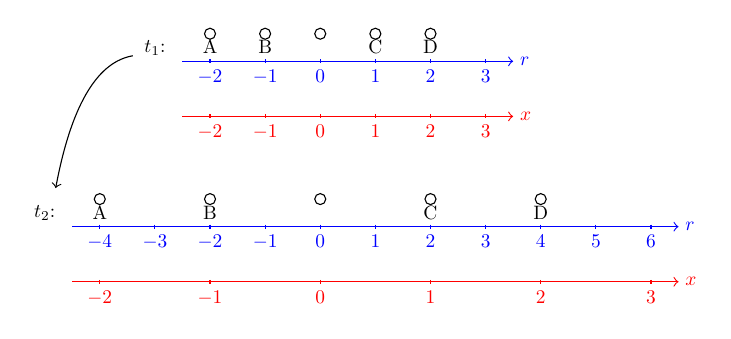
\begin{tikzpicture}[global scale = 0.7]
	\draw (-3, 1.5) circle(0) node[anchor=north] {$t_1$:};
	
	\draw (-2, 1.5) circle(0.1) node[anchor=north] {A};
	\draw (-1, 1.5) circle(0.1) node[anchor=north] {B};
	\draw (0, 1.5) circle(0.1) ;
	\draw (1, 1.5) circle(0.1) node[anchor=north] {C};
	\draw (2, 1.5) circle(0.1) node[anchor=north] {D};
	
	\draw[->,blue] (-2.5, 1) -- (3.5, 1);
	\foreach \x in {-2, -1, 0, 1, 2, 3} \draw[blue] (\x, 1cm + 1pt) -- (\x, 1cm - 1pt) node[anchor=north] {$\x$};
	\draw[blue] (3.5, 1) node[anchor=west] {$r$};
	
	\draw[->,red] (-2.5, 0) -- (3.5, 0);
	\foreach \x in {-2, -1, 0, 1, 2, 3} \draw[red] (\x, 1pt) -- (\x, -1pt) node[anchor=north] {$\x$};
	\draw[red] (3.5, 0) node[anchor=west] {$x$};
	
	
	
	\draw (-5, -1.5) circle(0) node[anchor=north] {$t_2$:};
	
	\draw (-4, -1.5) circle(0.1) node[anchor=north] {A};
	\draw (-2, -1.5) circle(0.1) node[anchor=north] {B};
	\draw (0, -1.5) circle(0.1) ;
	\draw (2, -1.5) circle(0.1) node[anchor=north] {C};
	\draw (4, -1.5) circle(0.1) node[anchor=north] {D};
	
	\draw[->,blue] (-4.5, -2) -- (6.5, -2);
	\foreach \x in {-4, -3, -2, -1, 0, 1, 2, 3, 4, 5, 6} \draw[blue] (\x, -2cm + 1pt) -- (\x, -2cm - 1pt) node[anchor=north] {$\x$};
	\draw[blue] (6.5, -2) node[anchor=west] {$r$};
	
	\draw[->,red] (-4.5, -3) -- (6.5, -3);
	\foreach \x in {-2, -1, 0, 1, 2, 3} \draw[red] (\x * 2, -3cm + 1pt) -- (\x * 2, -3cm - 1pt) node[anchor=north] {$\x$};
	\draw[red] (6.5, -3) node[anchor=west] {$x$};
	
	\draw[->] (-3.4, 1.1) .. controls (-4, 1) and (-4.5, 0.3) .. (-4.8, -1.3);
\end{tikzpicture}

\begin{itemize}
	\item 可建立一个相对于宇宙静止的坐标系$r$
	\item 除物理坐标系还可建立随宇宙不断膨胀的坐标系$x$(共动坐标系Comoving Coordinate)
\end{itemize}
\par 
可以看出物理距离等于共动距离乘以一个只与时间有关的因子$a(t)$,称为尺度因子
\begin{equation}
	r(t) = a(t) x
	\label{math:1}
\end{equation}
其中,$a(t)$描述宇宙在$t$时刻膨胀的速率,宇宙无中心,点点相同
\par 
结论:若CP始终成立,尺度因子只能是时间的函数,与空间无关;式\eqref{math:1}。
\begin{cnote}
	真实宇宙并非精确满足宇宙学原理,对均匀背景的偏离研究是宇宙学的重要研究方向
\end{cnote}

\subsection{Hubble定律及红移}
\subsubsection{Hubble定律}
\par 
由物理坐标系表达式\eqref{math:1}可计算出物理速度:
\begin{equation}
	v(t) = \frac{\dd a}{\dd t} x = \frac{\dot{a}}{a} a x = \frac{\dot{a}}{a} r \equiv H(t) r
\end{equation}
其中$H(t) = \frac{\dot{a}}{a}$为哈勃参数,当$t = t_0$,即当前时刻时,$H(t_0) = H_0$称为哈勃常数,是重要的待测参数。

\subsubsection{红移与尺度因子的关系}
\par 
哈勃定律中物理速度是通过红移测量计算的,当相对速度不大($v \ll c$),有$Z = \frac{v}{c}$
\par 
红移定义:$Z = \frac{\lambda_r - \lambda_e}{\lambda_e}$ $\Rightarrow$ $t_r$与$t_e$时刻光波长之比$\frac{\lambda_r}{\lambda_e} = 1 + Z$
\par 
考虑相距$\dd r$,相对速度$\dd v$的两个星系,$\dd v = \frac{\dot{a}}{a} \dd r$,红移为$\frac{\dd \lambda}{\lambda} = Z = \frac{\dd v}{c} = \frac{\dot{a}}{a} \frac{\dd r}{c} = \frac{\dot{a}}{a} \dd t = \frac{\dd a}{a}$,故$\lambda \propto a$,则$t_r$与$t_e$时刻的波长比:
\begin{equation}
	\frac{\lambda_r}{\lambda_e} = \frac{a(t_r)}{a(t_e)} = 1 + Z
	\label{math:2}
\end{equation}
若$t_r = t_0, a(t_0) \equiv 1$,则当前红移值$Z = \frac{1}{a(t_e)} - 1$,对于大爆炸($a = 0$),红移$Z \rightarrow \infty$;对于当前光,$Z = 0$

\begin{cnote}
	推导红移公式\eqref{math:2}时有假设两星系间距小,但实际上,用GR可严格导出对任意距离、任意宇宙几何的情况,波长(红移)与尺度因子都满足此公式
\end{cnote}

\begin{cbox}
	{宇宙膨胀的含义?}
	人不膨胀,因为化学键占主导;星系内,星体间引力作用占主导……实际上宇宙膨胀力密度很小
\end{cbox}
\begin{cbox}
	{退行速度超光速?}
	没有光到达,没有因果关系,不破坏因果律
\end{cbox}

\subsubsection{红移畸变效应}
\par 
星系的红移除了包括宇宙学红移,即星系发出的光子波长随背景宇宙的膨胀而拉长导致的红移,还包括星系本动速度造成的多普勒红移。假定我们拥有一个准确的宇宙学模型可以将星系红移正确地转化为星系与我们的距离,那么星系本动速度造成的多普勒红移会在星系的真实距离上叠加一个不可忽略的系统误差。导致观测到的星系三维位置其中一个维度 (视线方向上) 产生了“畸变”,导致我们观测到的星系空间分布呈现了各向异性的特征,即我们所说的“红移畸变效应”。
\par 
研究意义:星系本动速度大小反映了宇宙结构增长的快慢,所以通过测量星系红移巡天中的红移畸变效应可以帮助我们了解宇宙结构增长的历史,从而更好地甄别宇宙学模型和准确地限制模型参数。



\subsection{Friedmann方程}
\par 
引力势能:$V = - \frac{G M m}{r}$
\par 
模型:宇宙中均匀且各向同性地分布着质量密度为$\rho$的介质,由宇宙学原理知$\rho(t) = \sum_i \rho_i(t)$,任取一点作为原点建立物理坐标系,考虑处于$\vb*{r}$处质量为$m$的粒子,在此坐标系下受力为半径$r$的球给予的引力$M = \frac{4}{3} \pi r^3 \rho \Rightarrow V(r) = - \frac{4}{3} \pi G r^2 \rho m$ 
\par 
质点动能$T = \frac{1}{2} m \dot{r}^2$,故总能量$E = T + V = \frac{1}{2} m \dot{r}^2 - \frac{4}{3} \pi G r^2 \rho m = \text{const}$
\par 
$r(t) = a(t) x$是质点与观者之间的物理距离,代入得$E = \frac{1}{2} m \dot{a}^2 x^2 - \frac{4}{3} \pi G \rho m a^2 x^2$,化简得$\frac{2E}{m a^2 x^2} = (\frac{\dot{a}}{a})^2 - \frac{8}{3} \pi G \rho$
\par 
定义$\frac{2 E}{m x^2} =- k c^2$,其中$c$为光速,则代入得到\cword{Friedmann方程}:
\begin{equation}
	(\frac{\dot{a}}{a})^2 = \frac{8}{3} \pi G \rho - \frac{k c^2}{a^2} = (H(t))^2
	\label{math:3}
\end{equation}
其中$H(t)$为哈勃参数。

\par 
决定$a(t)$演化的有:宇宙介质的总密度$\rho$和常数$k$(其实就是曲率)
\par
若要满足宇宙学原理,空间曲率只有三种可能,如表\ref{table:1}所示。
\begin{table}[!h]
	\tiny
	\centering
	\begin{tabular}{|c|c|c|c|c|}
		\hline
		曲率$k$ & 几何             & 三角形内角和 & 圆周长 & 宇宙类型  \\ \hline
		$> 0$   & Spherical球空间   & $> \pi$      & $> 2 \pi r$  & Close \\ \hline
		$= 0$   & Flat平空间        & $= \pi$      & $= 2 \pi r$  & Flat  \\ \hline
		$< 0$   & Hyperbolic双曲空间 & $< \pi$      & $< 2 \pi r$  & Open  \\ \hline
	\end{tabular}
	\caption{三种空间性质对比}
	\label{table:1}
\end{table}

\par 
对Friedmann方程的讨论:
\begin{itemize}
	\item[1. ] $\rho(t)$是质量密度,其它地方可能会说是能量密度,差个$c^2$,没问题
	\item[2. ] $t = t_0$时,尺度因子$a(t_0) = 1$,$H_0^2 = \frac{8}{3} \pi G \rho_0 - k \quad(c = 1)$
	\item[3. ] 当$k = 0$,$\rho(t) = \frac{3 H_0^2}{8 \pi G} \equiv \rho_c(t)$称为临界密度 \\
	$\rho_c(t)$的物理意义:临界密度是使得宇宙刚好是平直几何的密度值 \\
	当前时刻$\rho_c(t_0) = \frac{3 H_0^2}{8 \pi G} = 1.88 h^2 \times 10^{-26} \mathrm{kg/m^3} = 2.78 h^2 \times 10^{11} M_{\text{Sun}} \mathrm{/Mpc^3}$,其中$H_0 = 100 h \quad \mathrm{km \cdot s^{-1} \cdot Mpc^{-1}}$,$h$是由实验待测的参数 \\
	$\rho_c(t)$还相当于200L的体积里有一个质子,而200L液态水里有$\sim 10^{29}$个质子 \\
	\begin{table}[!h]
		\tiny
		\centering
		\resizebox{\linewidth}{!}{
		\begin{tabular}{|c|c|c|c|c|}
			\hline
			时间   & 1990s                              & 现在                                                & 2010             & 2019                                                                \\ \hline
			项目 & \begin{tabular}[c]{@{}c@{}}Hubble space\\ Telescope key project\end{tabular}  & SHOES & Planck Satellite & \begin{tabular}[c]{@{}c@{}}HOLiCOW\\ arXiv: 1907.04869\end{tabular} \\ \hline
			$h$    & $0.72 \pm 0.08$      & $0.75 \pm 0.03$             & $0.673 \pm 0.012$   & $0.733 \pm 0.017$        \\ \hline
		\end{tabular}}
		\caption{$h$的测量}
		\label{table:2}
	\end{table}
	$h \sim 0.7$相当于100Mpc外的星体退行速度$\sim$ 7000km/s
	
	\item[4. ] 利用$\rho_c(t)$可定义一个无量纲密度常数$\Omega(t) = \frac{\rho(t)}{\rho_c(t)} \Rightarrow \rho = \Omega \rho_c = \Omega \frac{3 H^2}{8 \pi G}$ \\
	可以将Friedmann方程改写为$H^2 = H^2 \Omega - \frac{k}{a^2}$,即$\Omega = 1 + \frac{k}{H^2 a^2}$,$\Omega = 1$的宇宙称为临界密度宇宙 \\
	一般宇宙介质含多种类型,可定义相应的密度参数$\Omega = \Omega_{\text{mat}} + \Omega_{\text{rad}} + \cdots$ \\
	有时候也定义曲率的“密度参数”为$\Omega_k = - \frac{k}{a^2 H^2}$,从而Friedmann方程改写为$\Omega + \Omega_k = 1$
\end{itemize}


\subsection{热力学与流体方程}
\par 
单纯由Friedmann方程还不够解出$a(t)$,若将宇宙演化看作孤立系统,就可用热力学第一定律导出$\rho(t)$的另一个方程
\par 
考虑一个单位半径的共动球体,物理体积为$V = \frac{4}{3} \pi (ax)^3 = \frac{4}{3} \pi r^3$,总质量$m = \rho V$,总能量$E = m c^2 = \frac{4}{3} \pi a^3 \rho c^2$
\par 
该体积内宇宙介质在膨胀过程中满足热一:
\begin{equation}
	\dd E = T \dd S - p \dd V \overset{绝热}{=} - p \dd V 
\end{equation} 
而且我们有:
\begin{equation}
	\dv{E}{t} = \frac{4 \pi}{3} \qty(3 a^2 \dv{a}{t} \rho c^2 + a^3 \dv{\rho}{t} c^2 )
\end{equation}
以及$\dv{V}{t} = 4 \pi a^2 \dv{a}{t}$,综合三式可得:
\begin{equation}
	\dot{\rho} + 3 \frac{\dot{a}}{a} \qty(\rho + \frac{p}{c^2}) = 0
	\label{math:4}
\end{equation}
此方程即\cword{流体方程},这里可以发现我们又引入了新的未知量:压强$p(t)$
\par 
讨论:
\begin{itemize}
	\item[1. ] 导致宇宙介质能量变化的原因有两个:宇宙膨胀导致密度降低(括号里第一项)和体积膨胀介质通过压强对外做功(括号里第二项)
	\item[2. ] 由于宇宙学原理,宇宙各处压强均等,则$p(t)$不是$\vb*{x}$的函数且不存在压力$\grad{p} = 0$ \\
	做功损失的能量 $\Rightarrow$ 引力势能 $\Rightarrow$ 能量守恒
	\item[3. ] 目前有两个方程:Friedmann方程\eqref{math:3}和流体方程\eqref{math:4},联立可得\cword{加速度方程}
	\begin{equation}
		\frac{\ddot{a}}{a} = - \frac{4}{3} \pi G \qty(\rho + \frac{3p}{c^2})
		\label{math:6}
	\end{equation}
	注意该方程不独立,不含曲率$k$ \\
	$p>0, \rho >0 \Rightarrow \ddot{a} < 0$,故宇宙减速膨胀,要加速膨胀要求$p<0$(引入暗能量的动机)
\end{itemize}

\subsection{物态方程及宇宙介质的分类}
\par 
宇宙学中大多时候考虑最简单、最重要的\cword{物态方程}:
\begin{equation}
	p = \omega \rho c^2
	\label{math:5}
\end{equation}
其中,$\omega$是无量纲常量,不同介质$\omega$不一样:
$$
\omega = 
\begin{cases}
	0, \qq{非相对论性物质、无压物质(尘埃)} \\
	\frac{1}{3}, \qq{辐射、相对论性物质} \\ 
	-1, \qq{真空能或宇宙学常数(暗能量)}
\end{cases}
$$
\par 
将物态方程\eqref{math:5}代入流体方程\eqref{math:4},得到$\frac{\dot{\rho}}{\rho} = - 3 (1 + \omega) \frac{\dot{a}}{a}$,则有$\rho(a) \propto a^{-3 (1 + \omega)}$,对应上述三种情况我们有:
$$
\left\{
\begin{aligned}
	\rho_{\text{mat}} &\propto a^{-3} \qq{尘埃} \\
	\rho_{\text{rad}} &\propto a^{-4} \qq{辐射} \\
	\rho_{\Lambda} &= \text{const} \qq{宇宙真空能} \\
\end{aligned}
\right.
$$
\par 
下面给出一些物质粒子的分类:
\begin{table}[!h]
	\centering
	\scriptsize
	\begin{tabular}{|c|c|c|c|c|}
		\hline
		物质粒子    & 静质量/MeV         & 电荷 & 按速度大小分类                                                                                             & 宇宙介质类型                \\ \hline
		质子p     & 938.27          & 1  & \multirow{3}{*}{\begin{tabular}[c]{@{}c@{}}1. 最重要的重\\ 子物质\\ 2. 当前宇宙中\\ 最重要的非相\\ 对论性物质\end{tabular}} & \multirow{3}{*}{无压物质} \\[9pt] \cline{1-3}
		中子n     & 939.57          & 0  &                                                                                                     &                       \\[9pt] \cline{1-3}
		电子e     & 0.5110          & -1 &                                                                                                     &                       \\[9pt] \hline
		中微子$\mathrm{\nu}$   & $< 3\times 10^{-7}$ & 0  & 相对论性                                                                                                & 辐射                    \\ \hline
		光子$\mathrm{\gamma}$ & 0               & 0  & 相对论性                                                                                                & 辐射                    \\ \hline
		暗物质?    & ?               & 0  & \begin{tabular}[c]{@{}c@{}}1. 非量子类\\ 2. 相对论或\\ 非相对论性\\ 依赖于模型\end{tabular}                           & 依赖于模型                 \\ \hline
		暗能量     & -               & -  & -                                                                                                   & 能量                    \\ \hline
	\end{tabular}
	\caption{物质粒子分类表}
\end{table}

\subsubsection{宇宙介质的分类}
\par 
在宇宙学中,不同的宇宙介质是按照组成它们的基本粒子的性质分类的,可以根据粒子运动快慢分为:
\begin{itemize}
	\item[1. ] 非相对论性:$v \ll c$,此时$E = m_0 c^2 + \frac{p^2}{2 m_0}$ \\
		对于多粒子体系,可以根据$m_0 c^2$和$k_B T$之间的关系来区分,非相对论性有$m_0 c^2 \gg k_B T$
	\item[2. ] 相对论性:$m \simeq 0, v \simeq c, E \simeq pc$,例如光子
\end{itemize}

\begin{itemize}
	\item[1. ] 非相对论物质:特点:相互作用不频繁,可认为$p=0$无压 \\
	代表:重子物质 \\
	宇宙 $\leftarrow$ 原子 $\leftarrow$ 核子 $\leftarrow$ 夸克(p=uud, n=udd) \\
	稳定的重子只有质子和中子,故它们最重要 
	\begin{cnote}
		单个中子不稳定,$\tau \sim 15 \mathrm{min}$,与质子组成核的中子是稳定的
	\end{cnote}
	在宇宙学中,有时也把电子视为重子物质 \\
	宇宙电中性 $\Rightarrow$	电子数 = 质子数 \\
	在当前宇宙中,重子物质均为非相对论性的,非相对论性条件:对电子$T \ll 6 \times 10^9 \mathrm{K}$;对质子$T \ll 1 \times 10^{13} \mathrm{K}$ \\
	宇宙中重子物质原子大约有$\frac{3}{4} \mathrm{H}$、$\frac{1}{4} \mathrm{He}$和其它
	
	\item[2. ] 辐射物质:广义地说辐射是指所有相对论性的物质(例:重子物质若运动较快,如宇宙早期,也视作辐射)\\ 
	当前宇宙辐射的代表:光子和中微子
\end{itemize}

\subsubsection{光子}
\par 
$m = 0$且$E = \hbar \omega$,可以与其它粒子互相作用。若一盒光子气体到达平衡温度$T$,那么有如下结论:
\begin{itemize}
	\item[1. ] 平衡时频率介于$f$\textasciitilde$f$+$\dd f$,能量密度$\varepsilon(f) \dd f =\frac{8 \pi h}{c^3} \frac{f^3 \dd f}{\ee^{h f/k_B T } - 1}$,其中玻尔兹曼常数$k_B = 8.619 \times 10^{-5} \mathrm{eV/K} = 1.381 \times 10^{-23} \mathrm{J/K}$ \\
	$x \equiv \frac{h f}{k_B T}$,则$\varepsilon(f) = \frac{8 \pi (k_B T)^3}{c^3 h^2} \frac{x^3}{\ee^x - 1} \equiv \varepsilon(x)$,极值点$x_{\text{max}} \simeq 2.81$ \\
	$f_{\text{$\varepsilon$-peak}} \simeq 2.81 \frac{k_B T}{h}$,相应的光子能量$h f \simeq 2.81 k_B T$,则总能量主要是由$3 k_B T$左右的光子贡献
	
	\item[2. ] 光子气体的总能量密度$\varepsilon_{\gamma} = \int_{0}^{\infty} \varepsilon(f) \dd f = \frac{8 \pi (k_B T)^4}{c^3 h^3} \int_{0}^{\infty} \frac{x^3 \dd x}{\ee^x - 1} = \frac{8 \pi^5 (k_B T)^4 }{15 c^3 h^3}$ \\
	$\Rightarrow$ 温度为$T$时的光子气体总能量密度$\varepsilon_{\gamma} = \alpha T^4$,其中$\alpha \simeq 7.565 \times 10^{-16} \mathrm{J \cdot m^{-3} \cdot K^{-4}}$ \\
	又由$\rho_{\text{rad}} \propto a^{-4}$,以及$\varepsilon_{\text{rad}} = \rho_{\text{rad}} c^2 \propto a^{-4}$和$\varepsilon_{\text{rad}} \propto T^4$得到$T \propto a^{-1}$
	
	\item[3. ] 光子数密度按频率分布,频率$f$\textasciitilde$f$+$\dd f$,$n(f) = \frac{\varepsilon(f)}{h f} = \frac{8 \pi}{c^3} \frac{f^2}{\ee^x - 1} =  \frac{8 \pi (k_B T)^2}{c^3 h^2} \frac{x}{\ee^x - 1} $ \\
	极大值处$x \simeq 1.59$,$f_{\text{n-peak}} \simeq 1.59 \frac{k_B T}{h}$
	
	\item[4. ] 光子总粒子数密度$n_{\gamma} = \int_0^{\infty} n(f) \dd f = \frac{8 \pi (k_B T)^3}{c^3 h^3} \int_{0}^{\infty} \frac{x^2 \dd x}{\ee^x - 1} = \beta T^3$,其中$\beta \simeq 2.4041 \qty(\frac{k_B}{\hbar c})^3 \frac{1}{\pi^2} \simeq 2.029 \times 10^{7} \mathrm{m^{-3} \cdot K^{-3}}$,所以$n_{\gamma} \propto a^{-3}$
	
	\item[5. ] 光子平均能量$E_{\text{mean}} = \frac{E_{\text{tot}}}{N} = \frac{\varepsilon_{\gamma}}{n_{\gamma}} = \frac{\alpha}{\beta} T \simeq T \cdot 3.745 \times 10^{-23} \mathrm{J/K} \simeq 2.7 k_B T$
	
\end{itemize}

\par 
\textbf{小结:}
\begin{itemize}
	\item[1)] 平衡时仍有各频率的光子
	\item[2)] 不同频率光子的能量密度分布由黑体函数决定
	\item[3)] $\varepsilon(f)$在$f_{\text{$\varepsilon$-peak}} \simeq 2.81 \frac{k_B T}{h}$处取极大值 $\Rightarrow$ 对光子气体能量贡献最多的是$E = 2.81 k_B T$附近的光子,平均能量约为$2.7 k_B T$ 
\end{itemize}
\par 
\textbf{核心:}
\begin{itemize}
	\item[1)] 光子总能量密度$\varepsilon_{\gamma} = \alpha T^4$,总光子数密度$n_{\gamma} = \beta T^3$,单个光子平均能量$E_{\text{mean}} = \frac{\varepsilon_{\gamma}}{n_{\gamma}} \simeq 2.7 k_B T$
	\item[2)] $ \left.
	\begin{aligned}
		\varepsilon_{\text{CMB}} &\propto T^4 \\
		\rho_{\text{CMB}} &\propto a^{-4}
	\end{aligned}
	\right\}$
	$\Rightarrow$ $T_{\text{CMB}} \propto a^{-1}$
	
	\item[3)] $n_{\gamma} \propto a^{-3}$,对于非相对论物质,可证明也有数密度$n_{\text{matter}} \propto a^{-3}$ \\
	proof: $\rho_{\text{mat}} \propto \varepsilon_{\text{mat}} = n_{\text{mat}} E_{\text{sm}}$,其中$E_{\text{sm}}$为单个粒子的平均能量,故$\rho \propto a^{-3} \Rightarrow n \propto a^{-3}$
\end{itemize}

\begin{cbox}[red]
	{总粒子数密度是非常重要的,因为大多数时候粒子数守恒} 
	粒子间的相互作用可以导致粒子间的相互转化,因此当相互作用不频繁时$N$守恒;另一方面,相互作用很频繁时,$N$也应当守恒;只有当平衡破坏,有相互作用但不平衡时,$N$才不守恒。故大多数时候$N$守恒。 \\
	此时唯一导致粒子数密度变化的因素就是物理体积的变化$n = \frac{N}{V} \propto \frac{N}{a^3 x^3} \propto \frac{1}{a^3}$ \\
	\textbf{辐射和尘埃存在很多不同,但它们的数密度随$a$的演化行为相同,$n \propto a^{-3}$}
\end{cbox}

\begin{cnote}
	重要常数:常用单位$1 \mathrm{eV} = 1.602 \times 10^{-19} \mathrm{J}$ \\
	$k_B = 1.381 \times 10^{-23} \mathrm{J/K} = 8.619 \times 10^{-5} \mathrm{eV/K}$,$h \simeq 4.136 \times 10^{-15} \mathrm{eV \cdot s}$ \\
	$\alpha = \frac{\pi^2 k_B^4}{15 \hbar^3 c^3} = 7.565 \times 10^{-16} \mathrm{J \cdot m^{-3} \cdot K^{-4}}$(光子气体的总能量密度$\varepsilon_{\gamma} = \alpha T^4$) \\
	$\beta = \frac{2.4041}{\pi^2} \qty(\frac{k_B}{c \hbar})^3 = 2.029 \times 10^7 \mathrm{m^{-3} \cdot K^{-3}}$(光子气体的总光子数密度$n_{\gamma} = \beta T^3$)
\end{cnote}

\begin{itemize}
	\item[A] 应用:CMB \\
	观测表明,当前的CMB与温度为$T_0 = 2.7655 \pm 0.0006 K$的黑体辐射谱符合较好
	\begin{itemize}
		\item[1)] $\varepsilon_{\text{CMB}} = \alpha T_0^4 = 4.175 \times 10^{-14} \mathrm{J/m^3} = 0.2606 \mathrm{MeV/m^3}$ \\
		$\rho_{\text{CMB}} = \frac{\varepsilon_{\text{CMB}}}{c^2} = 4.639 \times 10^{-31} \mathrm{kg/m^3}$,进一步算出CMB光子的密度参数 \\
		$\Omega_{\text{CMB}} = \frac{\rho_{\text{CMB}}}{\rho_{\text{critical}}} = \frac{4.639 \times 10^{-31}}{1.88 h^2 \times 10^{-26}} \simeq 2.47\times 10^{-5} h^{-2} \quad (h \simeq 0.7)$ \\
		可见光子对临界密度的贡献很小
		\begin{cbox}
			{CMB光子和宇宙中恒星发出的光子哪个多?}
			当前星系亮度密度$\Psi \simeq 1.7 \times 10^{8} L_{\text{Sun}}/\mathrm{Mpc^{-3}} \simeq 2.2 \times 10^{-33} \mathrm{W/m^3}$,$\varepsilon_{\text{starlight}} \sim 0.006 \mathrm{MeV/m^3} \sim 2.3\% \varepsilon_{\text{CMB}}$(粗略估计) \\
			更为细致的研究表明:$\frac{\varepsilon_{\text{starlight}}}{\varepsilon_{\text{CMB}}} \simeq 0.1$,早期宇宙该值更小,故在计算宇宙光子能量密度时可近似忽略非CMB光子
		\end{cbox}
	
		\item[2)] 光子数密度为$n_{\text{CMB}} \simeq 4.107 \times 10^8 \mathrm{/m^3}$,相当于411个$\mathrm{/cm^3}$ \\
		$\Rightarrow$ CMB光的平均能量$E_{\text{mean}} \simeq 2.7 k_B T \simeq 6.344 \times 10^{-4} \mathrm{eV}$,平均频率$f_{\text{mean}} = \frac{E_{\text{mean}}}{h} \simeq 1.534 \times 10^{11} \mathrm{Hz}$,波长$\lambda = \frac{c}{f} \simeq 2 \mathrm{mm}$(微波波段)
	\end{itemize}

	\item[B] 应用:中微子(共三种$\nu_{e}$、$\nu_{\mu}$、$\nu_{\tau}$),它们的质量都很小$m < 3 \times 10^{-7} \mathrm{MeV/c^2}$ \\
	相互作用弱,很难探测,假设$m=0$ $\stackrel{\text{理论}}{\Longrightarrow}$ $\Omega_{\nu} \simeq 0.681 \Omega_{\text{CMB}}$ \\
	因此当前宇宙中辐射的密度参数$\Omega_{\text{rad}}{}_0 = \Omega_{\nu}{}_0 + \Omega_{\text{CMB}}{}_{0} \simeq 4.15 \times 10^{-5} h^{-2}$
\end{itemize}

\subsubsection{宇宙学常数$\Lambda$(最简单的暗能量模型)}
\begin{cbox}
	{何故引入$\Lambda$?}
	在宇宙学中的一个重要可观测常数:减速参数$q_0 \equiv - \frac{\ddot{a}(t_0)}{a(t_0)} \frac{1}{H_0} = - \frac{a(t_0) \ddot{a}(t_0)}{\qty(a(t_0))^2}$ \\
	于1990年代对\Rmnum{1}${}_a$型超新星研究发现$q_0 < 0, \ddot{a} > 0$,说明宇宙加速膨胀 \\
	然而,由加速度方程\eqref{math:6}可知无论是matter($p=0$)还是radiation($p = \frac{1}{3} \rho c$),必有$\ddot{a} < 0$,矛盾
\end{cbox}

\par 
为了解释宇宙加速膨胀,最简单的方式:假设宇宙不仅由尘埃和辐射组成,还有一种(等效)物质密度为常数的分量$\rho_{\text{tot}} = \rho + \rho_{\Lambda} = \rho_{\text{mat}} + \rho_{\text{rad}} + \rho_{\Lambda}$,其中$\rho_{\Lambda} \equiv \frac{\Lambda}{8 \pi G}$,相应的密度参数$\Omega_{\Lambda} = \frac{\Lambda}{8 \pi G} \frac{8 \pi G}{3 H^2} = \frac{\Lambda}{3 H^2}$是含时的
\begin{cnote}
	我们总是用$\rho = \rho_{\text{mat}} + \rho_{\text{rad}} $表示广义物质,其中$\rho_{\text{mat}}$代表非相对论物质,$\rho_{\text{tot}} = \rho + \rho_{\Lambda}$为宇宙介质总质量密度
\end{cnote}
宇宙密度参数$\Omega_{\text{tot}} \equiv \frac{\rho_{\text{tot}}}{\rho} = \Omega_{\text{mat}} + \Omega_{\text{rad}} + \Omega_{\Lambda}$,由于$\rho_{\Lambda}$为常数,由$\dot{\rho_{\Lambda}} + 3 \frac{\dot{a}}{a} \qty(\rho_{\Lambda} + \frac{p_{\Lambda}}{c^2}) = 0$ $\Rightarrow$ $p_{\Lambda} = - \rho_{\Lambda} c^2$,有负压,可以解释加速膨胀

\par 
含$\Lambda$的Friedmann方程$H^2 = \frac{8 \pi G}{3} \rho_{\text{tot}} - \frac{k c^2}{a^2}$或者写成$1 = \frac{8 \pi G}{3 H^2} \rho_{\text{tot}} - \frac{k c^2}{a^2 H^2} = \Omega_{\text{tot}} - \frac{k c^2}{a^2 H^2} = \Omega_{\text{tot}} + \Omega_k$

\par 
密度参数与宇宙几何的关系
$$
\left\{
\begin{aligned}
	0 < \Omega_{\text{tot}} < 1 \Rightarrow \Omega_k > 0 , k < 0 \qq{开放宇宙} \\
	\Omega_{\text{tot}} = 1 \Rightarrow \Omega_k = 0 , k = 0 \qq{平坦宇宙} \\
	\Omega_{\text{tot}} > 1 \Rightarrow \Omega_k < 0 , k > 0 \qq{封闭宇宙} 
\end{aligned}
\right.
$$
\
\begin{cbox}
	{$\Lambda$项可解释加速膨胀,物理上对应什么?}
	一种可能的解释是$\Lambda$是真空能,但是由粒子物理所预言的真空能远远大于$\Lambda$的观测值,该矛盾叫宇宙学常数问题 \\
	其它解释:精质(quintessence)模型,$\Lambda(t)$随时间缓变,物态方程一般只需要$\omega< - \frac{1}{3}$就可以解释加速膨胀
\end{cbox}
	
	\section{宇宙学的简单模型及其解}
	\subsection{简单宇宙模型}
\begin{equation}
	H^2 = \qty(\frac{\dot{a}}{a})^2 = \frac{8 \pi G}{3} \rho_{\text{tot}} - \frac{k c^2}{a^2}
\end{equation}
\begin{cnote}
	流体和物态方程对不同介质是分别成立的,但Friedmann方程的$\rho_{\text{tot}}$是所有介质的质量密度之和,一般分别讨论只含某种介质的情况
\end{cnote}

\subsubsection{空的宇宙$\rho_{\text{tot}}=0$}
\par 
此时Friedmann方程变为$H^2 = \qty(\frac{\dot{a}}{a})^2 = - \frac{k c^2}{a^2}$,则$\dot{a} = \sqrt{-k} c$,现在方程只有曲率了
\begin{itemize}
	\item[1)] $k > 0$ 无意义
	\item[2)] $k = 0, \dot{a} = 0, a = \text{const}$ 平直宇宙不膨胀,无物质,是平庸解
	\item[3)] $k < 0, a \propto t \stackrel{a(t_0)=1}{\Longrightarrow} a(t) = \frac{t}{t_0}, t_0 = \qty(\sqrt{-k} c)^{-1}$ 描述了一个虚无(empty)、负曲率、膨胀的宇宙,Milne宇宙(1930年E.A.Milne)
\end{itemize}

\subsubsection{$k=0$仅有一类宇宙介质}
\par 
此时Friedmann方程变为$\qty(\frac{\dot{a}}{a})^2 = \frac{8 \pi G}{3} \rho_{\text{tot}}$

\begin{itemize}
	\item[1)] 仅含有宇宙学常数$\rho_{\Lambda} = \frac{\Lambda}{8 \pi G} \Rightarrow H^2(t) = \qty(\frac{\dot{a}}{a})^2 = \frac{\Lambda}{3}, \Lambda > 0$,这说明尺度因子按指数变化$a(t) = \ee^{H_0 (t - t_0)}$ \\
	de Sitter宇宙(1917年W.de Sitter),没有物质,不能描述当前宇宙,但可以描述宇宙早期的暴涨阶段
	
	\item[2)] 对尘埃和辐射 \\
	有$\rho \propto a^{-3(1+\omega)}$,代入Friedmann方程得到$\qty(\frac{\dot{a}}{a})^2 \propto a^{-3(1+\omega)}$ $\Rightarrow$ $a(t) = \qty(\frac{t}{t_0})^{\frac{2}{3(1+\omega)}}, \rho(a(t)) = \rho(t) \propto t^{-2}$ \\
	具体地:(Einstein-de Sitter模型,1932年)
	\begin{itemize}
		\item[a.] 对尘埃,$\omega = 0$,$a(t) = \qty(\frac{t}{t_0})^{\frac{2}{3}}$,$\rho(t) = \rho_0 \qty(\frac{t}{t_0})^{-2}$
		\item[b.] 对辐射,$\omega = \frac{1}{3}$,$a(t) = \qty(\frac{t}{t_0})^{\frac{1}{2}}$,$\rho(t) = \rho_0 \qty(\frac{t}{t_0})^{-2}$
	\end{itemize}
\end{itemize}

\begin{table}[!h]
	\centering
	\scriptsize
	\resizebox{\linewidth}{!}{
	\begin{tabular}{|c|ccc|c|}
		\hline
		& \multicolumn{3}{c|}{$k=0$}                                                                                                                                                                                                 & $k<0$ \\ \hline
		& \multicolumn{1}{c|}{de Sitter}                                                   & \multicolumn{1}{c|}{Einstein-de Sitter}                                      & 纯辐射                                                      & Milne         \\ \hline
		宇宙组成   & \multicolumn{1}{c|}{\begin{tabular}[c]{@{}c@{}}只含$\Lambda$\\ $\omega=-1$\end{tabular}} & \multicolumn{1}{c|}{\begin{tabular}[c]{@{}c@{}}只含尘埃\\ $\omega=0$\end{tabular}} & \begin{tabular}[c]{@{}c@{}}只含辐射\\ $\omega=\frac{1}{3}$\end{tabular} & 只有负曲率         \\ \hline
		尺度因子 $a(t)$  & \multicolumn{1}{c|}{$a=\ee^{H_0(t - t_0)}$}                                                         & \multicolumn{1}{c|}{$a = \qty(\frac{t}{t_0})^{\frac{2}{3}}$}                                                       &      $a = \qty(\frac{t}{t_0})^{\frac{1}{2}}$       &    $a = \frac{t}{t_0}$   \\ \hline
		哈勃参数   & \multicolumn{1}{c|}{$H(t)=H(t_0)=\sqrt{\frac{\Lambda}{3}}$}                                                           & \multicolumn{1}{c|}{$H(t) = \frac{2}{3t}$}          &        $H(t) = \frac{1}{2t}$               &   $H(t) = \frac{1}{t}$   \\ \hline
		膨胀速度$v \propto \dot{a}$   & \multicolumn{1}{c|}{$v \propto \ee^{H_0 t}$}                                                           & \multicolumn{1}{c|}{$v \propto t^{-\frac{1}{3}}$}                                                       &               $v \propto t^{-\frac{1}{2}}$     &   $v = \text{const}$     \\ \hline
		减速参数$q = \frac{-\ddot{a}}{a H^2}$ & \multicolumn{1}{c|}{-1(加速)}                                                           & \multicolumn{1}{c|}{$\frac{1}{2}$(减速)}                                                       &    1(减速)            &    0(匀速自由膨胀)   \\ \hline
		$\rho(a)$ & \multicolumn{1}{c|}{常数$\frac{\Lambda}{8 \pi G}$}                                                           & \multicolumn{1}{c|}{$\propto a^{-3} \propto t^{-2}$}                                                       &                      $\propto a^{-4} \propto t^{-2}$    &   $a^{-2}$     \\ \hline
	\end{tabular}}
	\caption{简单宇宙模型表}
\end{table}

\subsection{多分量共存的宇宙学模型}
\subsubsection{平直时空,只含物质和辐射}
\par 
流体方程对不同分量分别成立,$\rho_{\text{mat}} \propto a^{-3}, \rho_{\text{rad}} \propto a^{-4}$,Friedmann方程中$\rho_{\text{tot}} = \rho_{\text{mat}} + \rho_{\text{rad}} \quad (\Lambda = 0)$难以解析求解
\par 
策略:考虑某一主导分量
\begin{itemize}
	\item[1)] 辐射主导$\rho_{\text{tot}} \simeq \rho_{\text{rad}}$,此时尺度因子行为$a(t) \propto t^{\frac{1}{2}}, \rho_{\text{rad}} \propto t^{-2} \Rightarrow \rho_{\text{mat}} \propto a^{-3} \propto t^{-\frac{3}{2}}$ \\
	随$t$增加,物质的质量密度衰减比辐射慢
	
	\item[2)] 物质主导$\rho_{\text{tot}} \simeq \rho_{\text{mat}}$,此时尺度因子行为$a(t) \propto t^{\frac{3}{2}}, \rho_{\text{mat}} \propto t^{-2} \Rightarrow \rho_{\text{rad}} \propto a^{-4} \propto t^{-\frac{8}{3}}$ \\
	仍然是辐射衰减快
\end{itemize}
\par 
故辐射主导不稳定而物质主导稳定,最终物质占主导地位

\subsubsection{更一般的情况}
\par
对于更一般的多分量共存宇宙,根据密度参数之间的关系(主要是$\Omega_0$和$\Omega_{\Lambda, 0}$的关系)
\par 
Friedmann方程$H^2 = \frac{8 \pi G}{3} (\rho + \rho_{\Lambda}) - \frac{k c^2}{a^2}, 1 = \frac{8 \pi G}{3 H^2} (\rho + \rho_{\Lambda}) - \frac{k c^2}{H^2 a^2} \Rightarrow 1 = \frac{\rho + \rho_{\Lambda}}{\rho_c} - \frac{k c^2}{a^2 H^2} \equiv \Omega + \Omega_{\Lambda} + \Omega_{k}$

\begin{itemize}
	\item 分类一:开放、封闭、平直 \\ 
	\cword[blue]{$\Omega_{\Lambda, 0} = 1 - \Omega_{0} + \frac{k c^2}{H_0^2}$},当$\Omega_{\Lambda, 0} = 1 - \Omega_{0}$时$k = 0$
	
	\item 分类二:由加速度方程$\frac{\ddot{a}}{a} = - \frac{4 \pi G}{3} \qty(\rho + \frac{3p}{c^2}) + \frac{\Lambda}{3}$以及减速参数定义$q = - \frac{\ddot{a}}{a H^2}$,可以得到$q H^2 = \frac{4 \pi G}{3} \qty(\rho + \frac{3p}{c^2}) - \frac{\Lambda}{3}$ \\
	考虑当前时刻(物质主导)$q_0^2 H_0^2 \simeq \frac{4 \pi G}{3} \rho_{\text{mat}, 0} - \frac{\Lambda}{3}$ \\ 故\cword[red]{$q_0 = \frac{4 \pi G}{3 H_0^2} \rho_0 - \frac{\Lambda}{3 H_0^2} = \frac{1}{2} \Omega_{0} - \Omega_{\Lambda, 0}$} \\
	若进一步考虑$k=0$情况,Friedmann方程退化为$\Omega + \Omega_{\Lambda} = 1, q_0 = \frac{3}{2} \Omega_0 - 1$,当$\Omega_{0} = \frac{2}{3}$时$q_0 = 0 \Rightarrow \Omega_{\Lambda, 0} > \frac{1}{3}$则加速膨胀
	
	\item 其它分类:1. 宇宙初始时刻\cword[magenta]{有无大爆炸};2. 宇宙\cword[green]{最终坍缩还是持续膨胀}
\end{itemize}

\begin{tikzpicture}[global scale = 1.3]
	
	\draw[->,black] (0, -1) -- (4, -1);
	\foreach \x in {1, 2, 3} \draw[black] (\x, -1cm - 1pt) -- (\x, -1cm + 1pt) node[anchor=north] {$\x$};
	\draw[black] (0, -1cm - 1pt) -- (0, -1cm + 1pt) node[anchor=north west] {$0$};
	\draw[black] (4.2, -1) node[anchor=west] {$\Omega_0$};
	\draw[->,black] (0, -1.5) -- (0, 4);
	\foreach \x in {-1, 0, 1, 2, 3} \draw[black] (-1pt, \x) -- (1pt, \x) node[anchor=east] {$\x$};
	\draw[black] (0, 4.2) node[anchor=east] {$\Omega_{\Lambda, 0}$};
	
	\draw[black] (0, 3) -- (3, 3);
	\foreach \x in {1, 2} \draw[black] (\x, 3cm - 1pt) -- (\x, 3cm + 1pt);
	\draw[black] (3, -1) -- (3, 3.5);
	\foreach \x in {-1, 0, 1, 2, 3} \draw[black] (-1pt + 3cm, \x) -- (1pt + 3cm, \x);

	\draw[blue] (0, 1) -- (2, -1);
	\draw[red] (0, 0) -- (3, 1.5);
	\draw[blue] (1, 0) node[anchor=north east, font=\fontsize{8}{8}] {开放};
	\draw[blue] (1, 0) node[anchor=south west, font=\fontsize{8}{8}] {封闭};
	\draw[red] (2, 1) node[anchor=north west, font=\fontsize{8}{8}] {减速};
	\draw[red] (2, 1) node[anchor=south east, font=\fontsize{8}{8}] {加速};
	
	\draw[magenta] (0, 1) .. controls (0.3, 2) and (0.5, 2.5) .. (1.3, 3);
	\draw[magenta] (0.6, 2.5) node[anchor=north west, font=\fontsize{6}{6}] {有大爆炸};
	\draw[magenta] (0.6, 2.5) node[anchor=south east, font=\fontsize{6}{6}] {无大爆炸};
	
	\draw[green] (0, 0) .. controls (1, 0.1) and (2, 0.25) .. (3, 0.45);
	\draw[green] (2.5, 0.3) node[anchor=north, font=\fontsize{6}{6}] {再坍缩};
	\draw[green] (2.5, 0.25) node[anchor=south east, font=\fontsize{6}{6}] {一直膨胀};

\end{tikzpicture}

\par 
可见$\Omega_{0}$和$\Omega_{\Lambda, 0}$是两个很关键的可观测量
\begin{cbox}
	{$\Omega_{0}$和$\Omega_{\Lambda, 0}$的观测值是多少?}
	当前关于超新星和CMB以及重子声学振荡(BAO)等多种观测已经把参数的可能取值限制在很小的范围内,$\Omega_{0} \simeq 0.3, \Omega_{\Lambda, 0} \simeq 0.7$ \\
	所以当前宇宙$k \simeq 0$,加速膨胀,存在大爆炸,持续膨胀,我们把$\Omega_{0} \simeq 0.3, \Omega_{\Lambda, 0} \simeq 0.7$叫做宇宙学标准模型,即Flat $\Lambda$CDM模型
\end{cbox}

\subsection{宇宙年龄}
\subsubsection{观测限制}
The age of the universe, 'Physics Reports', 307, (1998) 23-30, Review.
\begin{itemize}
	\item[1. ] 地质学限制:$T_{\text{地球}} \sim 50 \text{亿年}$
	\item[2. ] 核年代学研究星系盘中铀同位素相对值:大约有$T > 100 \text{亿年}$
	\item[3. ] 白矮星冷却曲线:大约有$T > 100 \text{亿年}$
	\item[4. ] 最佳方案:研究古老球状星团,得到$T \simeq 100  \textasciitilde 130 \text{亿年}$
\end{itemize}

\subsubsection{理论}
\begin{itemize}
	\item[1. ] Milne宇宙($\rho_{\text{tot}} = 0$)$a(t) = \frac{t}{t_0}, H(t) = \frac{1}{t}, v(t) = \text{const}$,宇宙从$t=0, a(0) = 0$开始匀速膨胀到$a(t_0) = 1$的状态,得到宇宙年龄$\frac{1}{H_0}$约为140亿年($h \simeq 0.7$)
	\item[2. ] 物质与辐射混合$k = \Lambda = 0$,辐射比物质衰减得快 $\Rightarrow$ 宇宙演化中大多数时间物质主导$\frac{\dot{a}}{a} = H(t) = \frac{2}{3t}$,故有宇宙年龄约为$t_0 = \frac{2}{3H_0} \simeq 93 \text{亿年}$
	\item[3. ] Flat $\Lambda$CDM模型$\Omega + \Omega_{\Lambda} = 1$ \\
	Friedmann方程$H^2 = \frac{8 \pi G}{3} \rho_{\text{tot}} = \qty(\frac{\dot{a}}{a})^2, \rho_{\text{tot}} = \rho + \rho_{\Lambda} \simeq \rho_{\text{mat}} + \rho_{\Lambda} = \rho_0 a^{-3} + \rho_{\Lambda} \Rightarrow \dot{a}^2 = \frac{8 \pi G}{3} (\rho_0 a^{-1} + \rho_{\Lambda, 0} a^{2}) = H_0^2 (\Omega_0 a^{-1} + \Omega_{\Lambda, 0} a^2)$ \\
	$\dot{a} = H_0 \sqrt{\Omega_0 a^{-1} + \Omega_{\Lambda, 0} a^2}$积分得到$\int_{0}^{T} \dd t = \frac{2}{3 H_0} \frac{\arctan \sqrt{1-\Omega_{0}}}{\sqrt{1-\Omega_{0}}} \simeq 0.964 t_H \simeq 1.3456 \times 10^{10} \text{年}$
	
\end{itemize}


\subsection{暗物质}
\par 
$\Omega_{0} = 0.3$,占宇宙30\%的非相对论物质不全是重子物质
\subsubsection{重子物质的占比}
\begin{cbox}
	{发光恒星的质量密度占$\rho_c$的多少?}
	恒星的结构理论:由恒星的温度亮度$\Rightarrow$估算出质量,若观测足够大的区域$\Rightarrow$估算区域内恒星质量密度 \\
	研究结论(Ryden, P126):$\Omega_{\text{Star}, 0} \simeq 0.003$,只占$\Omega_{0}$的1\%
\end{cbox}


\subsubsection{恒星之外的重子物质}
\par
是否所有的重子物质都以恒星形式存在?
\begin{itemize}
	\item[1. ] MACHOs(massive compact halo objects 大质量致密晕天体) \\
	它们是一些低质量的恒星(发出的光太微弱探测不到),如褐矮星($M < 0.08 M_{\text{Sun}}$)或恒星尺度的小型黑洞,这些天体一般通过引力透镜效应进行观测 \\
	但即使考虑了MACHOs,对$\Omega_{\text{Star}, 0}$的估值也低于0.005,因此可作为DM的一部分但不会是全部
	\item[2. ] 星系气体 \\
	不仅存在于各个星系内(e.g.银河系或M31星系气体的质量是恒星质量的20\%),还大量存在于星系团内(e.g.在距离银河系100Mpc处的Coma Cluster后发座星系团,其恒星总质量$M_{\text{Comma star}} \simeq 2 \times 10^{13} M_{\text{Sun}}$,但该星系团内存在大量温度极高的星际气体$T \sim 10^8 \mathrm{K}$,可用X射线望远镜看到,对这些气体的研究给出$M_{\text{Comma gas}} \simeq 2 \times 10^{14} M_{\text{Sun}}$,是恒星质量的10倍) \\
	星际气体也存在于星系、星系间之外的广阔的星际空间中,这部分气体占总重子数的85\%!但它们密度极低,温度极低,目前技术很难对它们直接测量
\end{itemize}

\par 
CMB的观测结果和原初核合成理论限制:$0.021 \leqslant \Omega_{B} h^2 \leqslant 0.025$,若取$h = 0.7$,则$\Omega_{B} \in \qty[0.043, 0.051]$,仅有4\% \textasciitilde 5\%是重子物质,剩下25\%是非重子物质

\par 
结论:
\begin{itemize}
	\item[1. ] 发光天体只占重子物质的10\%左右
	\item[2. ] 绝大多数重子物质不以恒星的形式存在,暗重子物质主要以星际气体形式存在,占总密度的4\%
	\item[3. ] 宇宙中绝大多数的物质不仅不发光,而且不是重子物质,统称为暗物质
\end{itemize}

\subsubsection{暗物质存在的其它证据}
\begin{itemize}
	\item[1. ] 星系内存在DM(首次1914年Slipher) \\
	理论上,由向心力公式和万有引力公式得到速度$v = \sqrt{\frac{G M(R)}{R}}$,当$R$较大时,$M(R) \leftarrow \text{const}$,故$v \propto R^{- \frac{1}{2}}$ \\
	则Keplerian转动,$v$将衰减,而对M31等漩涡星系的观测表明(星系旋转曲线),$R$很大时$v$趋近于常数,这表明星系中有大量暗物质,实测速度比理论速度高3倍以上$\Rightarrow M_{\text{DM}} \simeq 10 M_{\text{star}}$
	
	\item[2. ] 星系团内也存在DM(首次1933年Zwicky) \\
	仍以Coma Cluster为例,一般有3种方法可以估算出星系团的总质量:
	\begin{itemize}
		\item[1)] 质点系的位力定理可以算出$M_{\text{coma}} \simeq 2 \times 10^{15} M_{\text{Sun}}$
		\item[2)] 高温气体辐射压与星系团自引力平衡也可推算出$M_{\text{coma}} \simeq 1.3 \times 10^{15} M_{\text{Sun}}$
		\item[3)] 引力透镜,结果一致
	\end{itemize}

	\item[3. ] 结构形成:1980s人们意识到重子物质不足以提供形成当前观测结构的引力,需要引入暗物质
\end{itemize}

\par 
主流观点认为,DM是由一种新型的与重子物质相互作用极弱的非重子物质构成,通常还假设这些物质缺乏使之形成盘状结构的耗散机制$\Rightarrow$DM形成球状晕结构 \\
\resizebox{\linewidth}{!}{$
	$$
	\Omega_{\text{tot}} 
	\begin{cases}
		\Omega_{\text{mat}} \sim 0.3 \rightarrow 
		\begin{cases}
			\Omega_{\text{DM}} = 0.2 \textasciitilde 0.25 \\
			\text{核合成} \Omega_{B} = 0.04 \textasciitilde 0.05 
			\begin{cases}
				\Omega_{\text{star}} = 0.005 \textasciitilde 0.01 \\
				\Omega_{\text{non-star}} = 0.04 \textasciitilde 0.05 (\text{星际气体})
			\end{cases} 
		\end{cases} \\
		\Omega_{\text{rad}} \sim 10^{-5} \\
		\Omega_{\Lambda} \sim 0.7
	\end{cases}
	$$
$}

\subsubsection{暗物质可能是什么?}
\begin{itemize}
	\item[A] 基本粒子说:
	\begin{itemize}
		\item[1. ] 我们已知的基本粒子,但对其性质不确定,如中微子 \\
		轻中微子,作为热暗物质,但不能很好解释宇宙结构形成(只可能作为一小部分) \\
		重中微子,作为冷暗物质,大多数阶段非相对论性
		\item[2. ] 超越标准模型的基本粒子,如BSM(超对称)中最轻的超对称伙伴(LSP) \\
		LSP取决于模型,LSP是WIMPs(Weak Interacting Massive Particles)的一类 \\
		另一类WIMPs例子:额外维中的Kaluza-Klein粒子
	\end{itemize}

	\item[B] 致密天体说:
	\begin{itemize}
		\item[1. ] 原初黑洞(Primordial Black Holes),前提:形成原初黑洞原在核合成之前
		\item[2. ] MACHOs,但丰度不足以解释星系晕的形成,对其探测的主要手段是引力透镜
	\end{itemize}
\end{itemize}
\subsubsection{暗物质探测法}
\begin{itemize}
	\item[1. ] 粒子对撞机
	\item[2. ] 基于暗物质湮灭
	\item[3. ] 暗物质与固体、液体的散射:与核碰撞散射 
	$$\begin{cases}
		\text{电信号:GaAs} \\
		\text{光信号:NaI} \\
		\text{热信号:产生声子进行探测}
	\end{cases}$$
\end{itemize}
	
	\section{热历史}
	\subsection{CMB的起源}
\par 
回顾:CMB的性质,CMB有平衡光子气的性质,观测得到$T_0 = 2.725 \mathrm{K}$
\begin{itemize}
	\item[1. ] CMB光子的总能量密度$\varepsilon_{\text{CMB}, 0} = \alpha T^4 \simeq 4.175 \times 10^{-14} \mathrm{J/m^3} = 0.2606 \mathrm{MeV/m^3}$
	\item[2. ] CMB密度参数$\Omega_{\text{CMB}, 0} = \frac{\rho_{\text{CMB}, 0}}{\rho_{\text{c}, 0}} = \frac{\varepsilon_{\text{CMB}, 0}}{\rho_{\text{c}, 0} c^2} \simeq 2.47 \times 10^{-5} h^{-2}$,一般可忽略
	\item[3. ] 光子的总粒子数密度$n_{\gamma} = \beta T^3 \simeq 4.107 \times 10^8 \mathrm{/m^3}$
	\item[4. ] 光子平均能量$E_{\text{mean}} = 2.7 k_B T \simeq 6.344 \times 10^{-4} \mathrm{eV}, \quad f = \frac{E_{\text{mean}}}{h} \simeq 1.534 \times 10^{11} \mathrm{Hz}$,波长大约2mm,属于微波
\end{itemize}

\begin{cbox}
	{黑体谱是平衡光子气体的性质,当前时刻CMB光子是否处于平衡}
	不是,CMB是早期宇宙遗留下来的,其形成后自由传播至今,是一种遗迹,因此有早期宇宙的关键信息
\end{cbox}

\subsubsection{早期宇宙与原子的电离}
\par 
$\rho_{\gamma} \propto a^{-4}$,结合$\varepsilon_{\gamma} = \alpha T^4$可以得到$T \propto a^{-1}$,故早期光子气体温度极高 
\par 
例子:取$a = 10^{-6}$时,CMB光子温度$T \simeq 3 \times 10^{6} \mathrm{K}$,此时$E_{\text{mean}} = 2.7 k_B T \simeq 3 k_B T \simeq 700 \mathrm{eV}$,远大于氢原子的电离能$I = 13.6 \mathrm{eV}$
\par 
简单起见,近似认为宇宙中所有的重子物质全是氢原子,那么每一个能量高于$I$的光子就可以将一个氢原子电离掉,如果高能光子的数目远多于氢原子数,则宇宙中所有的氢原子将被全部电离,宇宙将处于完全电离的状态,只有自由的电子、质子、光子而没有原子
\\
\textbf{宇宙中光子和氢原子的粒子数之比}
\par 
由核合成结论$0.021 \ll \Omega_{\text{B}, 0} h^2 \ll 0.025$,取中间值$\Omega_{\text{B}, 0} \equiv \frac{\varepsilon_{\text{B}, 0}}{\rho_{\text{c}, 0} c^2} \simeq 0.023 h^{-2}$ 
\par 
由此知$\varepsilon_{\text{B}, 0} = \Omega_{\text{B}, 0} \rho_{\text{c}, 0} c^2 \simeq 241.5 \mathrm{MeV/m^3}$,自由质子或中子的质量939MeV,可知$n_{\text{B}, 0} = 0.26 \mathrm{m^{-3}}$
\par 
而光子$n_{\gamma, 0} = 4.11 \times 10^8 \mathrm{m^{-3}}$,所以光子与重子数密度之比$\frac{n_{\gamma, 0}}{n_{\text{B}, 0}} = 1.6 \times 10^9$,有时也用重子——光子数之比$\eta \equiv \frac{n_{\text{B}, 0}}{n_{\gamma, 0}} \simeq 6 \times 10^{-10}$

\par 
前面说过,宇宙大多数时刻粒子数守恒,因此$\eta$值在早期宇宙也成立,因此极早期H原子可被完全电离

\subsubsection{Thomson散射与平衡态的建立}
\par 
自由电子与光子的相互作用$\gamma + \ee^{-} \rightarrow \gamma + \ee^{-}$
\par 
散射截面为$\sigma_{\ee} = 6.65 \times 10^{-29} \mathrm{m^2}$,是常数
\par 
光子平均自由程:平均而言一个光子在与$\ee^{-}$碰前走的距离$d = \frac{1}{n_{\ee} \sigma_{\ee}}$
\par 
光子平均碰撞时间:平均而言一个光子在碰到一个电子前所经历的时间$\frac{d}{c}$
\par 
光子与电子发生Thomson散射的速率(单位时间内发生散射的次数):
\begin{equation}
	\Gamma = \frac{c}{d} = n_{\ee} \sigma_{\ee} c
\end{equation}
\par 
在原子完全电离时,$n_{\ee} = n_{\mathrm{p}} \simeq n_{\mathrm{B}}$,因此有$n_{\ee} \simeq n_{\mathrm{B}} = n_{\mathrm{B}, 0} a^{-3}, n_{\mathrm{B}, 0} \simeq 0.26 \mathrm{m^{-3}}$
\par 
故有$\Gamma = n_{\ee} \sigma_{\ee} c = \frac{ n_{\mathrm{B}, 0} \sigma_{\ee} c}{a^3} \simeq 5.187 \times 10^{-21} a^{-3} \mathrm{s^{-1}}$
\par 
例如当$a = 10^{-6}$时,$\Gamma = 5.187 \times 10^{-3} \mathrm{/s}$
\par 
当$\Gamma \gg H$,就称光子与电子是耦合的,相互作用频繁,能达到平衡,有相同的$T$
\par
$\ee^{-}$与p也有相互作用,处于平衡$T$相同$\Rightarrow$光子气体的$T$就是整个宇宙的温度
\par 
由于$\gamma$与$\ee^{-}$之间有相互作用,此时的宇宙是不透明的

\subsubsection{光子与电子退耦合(decoupling)与CMB的形成}
\par 
当$\Gamma \ll H$时,认为$\gamma$与$\ee^{-}$几乎不相互作用,光子从与$\ee^{-}$频繁碰撞到几乎不发生作用的过程叫做退耦。退耦后,宇宙变成透明的,$\gamma$开始向各个方向自由传播,形成CMB





\par 
$\Gamma = H$是光子是否退耦的分界线,已知碰撞速率与尺度因子的关系$\Gamma = \frac { 5.187 \times 10 ^ { - 21 } / \mathrm{s} } { a ^ { 3 } }$,只要能找到$H$和$a$的关系,就可以算出$\Gamma = H$所对应的尺度因子的值$a_{\text{dec}}$
\par 
当前宇宙$\rho_{\text{mat}} \gg \rho_{\text{rad}}$,但由关系式$\rho_{\text{mat}} = \rho_{\text{mat}, 0} a^{-3}, \rho_{\text{rad}} = \rho_{\text{rad}, 0} a^{-4}$可以看出宇宙早期有$\rho_{\text{rad}} \gg \rho_{\text{mat}}$,则在某一时刻有$\rho_{\text{mat}} = \rho_{\text{rad}}$,相应尺度因子$a_{\text{eq}} = 	\frac{\rho_{\text{rad}, 0}}{\rho_{\text{mat}, 0}} \simeq \frac{4.15 \times 10^{-5} h^{-2}}{0.3} \simeq 2.8 \times 10^{-4}$

\begin{itemize}
	\item[1. ] 辐射主导,$a < a_{\text{eq}}$ \\
	Friedmann方程变为$H^2 = \frac{8 \pi G}{3} \rho_{\text{rad}}$或$\frac { H ^ { 2 } } { H _ { 0 } ^ { 2 } } = \frac { 8 \pi G \rho_{\text{rad}, 0} } { 3 H _ { 0 } ^ { 2 } a^4}  = \frac { \Omega _ { \text{rad}, 0 } } { a ^ { 4 } }$,因此辐射主导期的哈勃参数为$H = H_0 \sqrt{\Omega_{\text{rad}, 0}} a^{-2} = 100 h \mathrm{km \cdot s^{-1} \cdot Mpc^{-1}} \frac{\sqrt{4.15 \times 10^{-5} h^{-2}}}{a^2} = 2.14 \times 10^{-20} a^{-2} \mathrm{s^{-1}}$ \\
	当$a = 10^{-6}$时,$H = 2.14 \times 10 ^ { - 8 } \mathrm{s ^ { - 1 }} \ll \Gamma = 5.187 \times 10 ^ { - 3 } / \mathrm{s}$,这说明此时光子与电子和质子是耦合在一起的 \\
	当$a = 10^{-5}$时,$H = 2.14 \times 10 ^ { - 10 } \mathrm{s ^ { - 1 }} \ll \Gamma = 5.187 \times 10 ^ { - 6 } / \mathrm{s}$,光子仍未退耦合
	
	\item[2. ] 物质主导,$a > a_{\text{eq}}$,同样操作
\end{itemize}

\par 
假设宇宙在其膨胀过程中始终保持完全电离的状态,则由$\Gamma = \frac { 5.187 \times 10 ^ { - 21 } / \mathrm{s} } { a ^ { 3 } }$可以计算出退耦所对应的尺度因子和温度分别为$a \simeq 0.0254, T \simeq 100 \mathrm{K}$(需要考虑辐射主导向物质主导的转变)

\par 
这一估计忽略了一个重要的因素,即当温度足够低使得电子和质子可以形成中性的氢原子而能够将氢原子电离的高能光子已经不多时,由于自由电子的减少,光子将迅速退耦,所以退耦是在中性原子的形成之后迅速完成的

\par 
电子与质子结合形成中性氢原子的阶段叫做复合(recombination)时期,大概发生在宇宙温度$T_{\text{rec}} = 3760 \mathrm{K}$,或宇宙年龄$t_{\text{rec}} = 250000 \text{年}$时
\par 
光子与电子的退耦发生在复合时期之后,$T_{\text{dec}} = 2970 \mathrm{K}, t_{\text{dec}} = 350000 \text{年}$

\subsection{复合与退耦}
\subsubsection{Saha方程}
\par 
在$T \gtrsim 1 \mathrm{eV}$,光子与重子通过$\gamma + \mathrm{H} \rightleftharpoons \mathrm{p} + \ee^{-}$达到平衡 \\
为了定量地描述有多少中性H原子被电离,引入电离度$X$
\begin{equation}
	X = \frac{n_{\text{p}}}{n_{\text{B}}} = \frac{n_{\text{p}}}{n_{\text{H}} + n_{\text{p}}} \xlongequal[]{n_{\text{p}} = n_{\ee}} \frac{n_{\ee}}{n_{\ee} + n_{\text{H}}}
\end{equation}
\par 
$X = 1$表示重子被完全电离$n_{\text{H}} = 0$,$X = 0$表示重子全是中性原子,可证明$\frac{1 - X}{X^2} = \frac{n_{\text{H}}}{n_{\ee}^2} n_{\text{B}}$,再利用$n_{\text{B}} = \eta n_{\gamma} = \eta \beta T^{3}$,如何把$\frac{n_{\text{H}}}{n_{\ee}^2}$表示成$T$的函数?
\par 
对于H,p,$\ee^{-}$均有$m c^2 \gg k_{\text{B}} T$,它们都可以当做非相对论的,由统计物理知,非相对论的总粒子数密度$n_{x} = g_x \qty(\frac{m_x k_{\text{B}} T}{2 \pi \hbar^2})^{\frac{3}{2}} \exp(\frac{-m_x c^2 + \mu_x}{k_{\text{B}} T}),\quad x = \text{H}, \text{p}, \ee^{-}$,其中$\mu_x$为化学势
\par 
化学平衡条件$\mu_{\text{H}} = \mu_{\ee} + \mu_{\text{p}}$得到,$\frac{n_{\text{H}}}{n_{\text{p}} n_{\ee^{-}}} = \frac{g_{\text{H}}}{g_{\ee} g_{\text{p}}} \qty(\frac{m_{\text{H}}}{m_{\ee} m_{\text{p}}} \frac{2 \pi \hbar^2}{k_{\text{B}} T})^{\frac{3}{2}} \ee^{-\beta (m_{\text{H}} -m_{\text{p}} - m_{\ee^{-}}) c^2}$
\par 
由电中性$n_{\text{p}} = n_{\ee}$,电离能$I = (-m_{\text{H}} +m_{\text{p}} + m_{\ee^{-}}) = 13.6\mathrm{eV}$,$\frac{m_{\text{H}}}{m_{\ee} m_{\text{p}}} \simeq \frac{1}{m_{\ee}}$,$g_{\text{p}} = g_{\ee^-} = 2, g_{\text{H}} = 4$得到\cword{Saha方程}:

\begin{equation}
	\frac{n_{\text{H}}}{n_{\ee}^2} = \qty(\frac{2 \pi \hbar}{m_{\ee} k_{\text{B}} T})^{\frac{3}{2}} \ee^{\frac{I}{k_{\text{B}}T}}
\end{equation}


\par 
将Saha方程代入电离度的方程得到
\begin{equation}
	\frac{1 - X}{X^2} = 3.8 \eta \qty(\frac{k_{\text{B}}T}{m_{\ee}c^2})^{\frac{3}{2}} \ee^{\frac{13.6 \mathrm{eV}}{k_{\text{B}}T}} \equiv S(T)
\end{equation}
其中$\eta \equiv \frac{n_{\text{B}, 0}}{n_{\gamma, 0}} = 6 \times 10^{-10}$,等价地有$X(T) = \frac{-1 + \sqrt{1 + 4 S(T)}}{2 S(T)}$

\subsubsection{复合}
\par 
Liddle书中定义$T_{\text{rec}}$对应的$X = 0.1$,90\%的电子与质子形成H原子$\Rightarrow$ $k_{\text{B}} T_{\text{rec}} = 0.3 \mathrm{eV}, T_{\text{rec}} \approx 3600 \mathrm{K}$
\par 
Ryden定义$X=0.5$ $\Rightarrow$ $k_{\text{B}} T_{\text{rec}} = 0.324 \mathrm{eV} = \frac{I}{42}, T_{\text{rec}} = 3760 \mathrm{K}$,复合能标0.3eV小于$I = 13.6 \mathrm{eV}$

\par 
由红移和$a$之间的关系$1 + Z = \frac{1}{a(t)}$,又知$a \propto T^{-1}$,故$T = (1 + Z) T_0$,代入$T_0 = 2.7 \mathrm{K}$,得到$Z_{\text{rec}} \approx 1320$,而辐射——物质等量期红移为$Z_{\text{eq}} \simeq 3500$,故复合(以及其后的退耦)发生于物质主导期

\par 
物质主导$a(t) = \qty(\frac{t}{t_0})^{\frac{2}{3}}$,由$T \propto a^{-1}$可知$t_{\text{rec}} = \frac{t_0}{(1 + Z_{\text{rec}})^{\frac{3}{2}}} \sim 29 \text{万年}$

\subsubsection{退耦}
\par 
定义光子的退耦发生于$\Gamma \simeq H$时,其中$\Gamma = n_{\ee} \sigma_{\ee} c$,只有$n_{\ee}$会变化,影响$n_{\ee}$的两个因素:1. 宇宙膨胀;2. 复合过程
\par 
由电离度定义$X = \frac{n_{\text{p}}}{n_{\text{B}}} = \frac{n_{\text{e}}}{n_{\text{B}}}$,得到$n_{\ee} = X n_{\text{B}} = X \eta n_{\gamma} = X \eta \beta T^3$,所以有$\Gamma = (X \eta \beta T^3) \sigma_{\ee} c$
\par 
为了与$\Gamma$相比较,也要将$H$写成$T$的函数,退耦发生于物质主导期,相应的Friedmann方程为$\frac{H^2}{H^2_0} = \frac{8 \pi G}{3 H_0^2} \rho_{\text{mat}} = \frac{\rho_{\text{mat}, 0}}{\rho_{\text{c}, 0}} a^{-3} = \Omega_{ \text{mat}, 0 } a^{-3}$
\par 
所以$H = H_0 \frac{\sqrt{\Omega_{ \text{mat}, 0 }}}{a^{\frac{3}{2}}}$,由$a \propto T^{-1}, aT = a_0 T_0$,得到$H = H_0 \sqrt{\Omega_{ \text{mat}, 0 }} \qty(\frac{T}{T_0})^{\frac{3}{2}}$
\par 
因此$\Gamma = H \Rightarrow X(T_{\text{dec}}) T_{\text{dec}}^{\frac{3}{2}} = \frac{H_0 \sqrt{\Omega_{ \text{mat}, 0 }}}{\eta \beta \sigma_{\ee} c T_0^{\frac{3}{2}}}$,最终得到$T_{\text{dec}} \simeq 3060 \mathrm{K}$
\par 
退耦后,光子自由传播至今,形成了CMB,重子物质几乎不再与光子发生相互作用,它们不再同温

\par
CMB光子形成时,其温度大概是3000K,随着宇宙的膨胀,最终冷却到温度为3K的黑体辐射,过程中,光子数密度减少,每个光子的频率都将红移,光子气体的温度下降,但是黑体分布函数保持不变,仍保持黑体谱

\par 
目前在地球上观测到的CMB光子都来自一个以地球为中心,半径约为$ 6000 h^{-1} $Mpc的球面,称为最终散射面,宇宙中任何观者都有在与之相应的最终散射面(surface of last scattering)

\subsection{宇宙膨胀与黑体谱的保持}
\par 
CMB形成后,光子不再发生相互作用,光子数守恒,宇宙膨胀会影响CMB的三个性质:
\begin{itemize}
	\item[1. ] 数密度减少,$n \propto a^{-3}$
	\item[2. ] 每个光子的频率都将发生红移$f \propto a^{-1}$
	\item[3. ] 光子气体的温度下降$T \propto a^{-1}$
\end{itemize}
\par 
考虑$a \rightarrow a'$的过程,$a$时,频率介于$f$\textasciitilde$f + \dd f$内光子的数密度为$n(f) \dd f = c \frac{f^2 \dd f}{\ee^{\frac{h f}{k_{\text{B}}T}} - 1}$;$a'$时,频率$f \rightarrow f'  = f\frac{a}{a'}$,相应的数密度变为$n(f') \dd f' = n(f) \dd f \qty(\frac{a}{a'})^3 = c \frac{f^2 \dd f}{\ee^{\frac{h f}{k_{\text{B}}T}} - 1} \qty(\frac{a}{a'})^3 = c \frac{f'^2 \dd f'}{\ee^{\frac{h f'}{k_{\text{B}}T'}} - 1}$,故$a'$时仍为黑体谱,CMB是一种遗迹

\subsection{$a,T,E,Z,t$之间的换算关系}
\par 
由$a \propto T^{-1}$及红移$a$的关系知$1 + Z = \frac{a_0}{a} = \frac{T}{T_0}$或$a = \frac{1}{1 + Z}, T = (1 + Z) T_0$,能征能量$E \simeq k_{\text{B}} T$
\par 
例如,对物质——辐射等量期$a_{\text{eq}} = \frac{\rho_{\text{rad}, 0}}{\rho_{\text{mat}, 0}} \simeq \frac{1}{3500}$,换成其它标尺$T_{\text{eq}} = \frac{2.725 \mathrm{K}}{a_{\text{eq}}} = 9600 \mathrm{K} \approx 10^4 \mathrm{K}$,$E_{\text{eq}} = k_{\text{B}} T \simeq 2.8 \mathrm{eV} \approx 1 \mathrm{eV}$,$Z_{\text{eq}} = \frac{1}{a_{\text{eq}}} -1 \approx 3500$

\par 
$T$,$E$,$Z$与$a$之间的转换关系与$a(t)$的具体解无关,但若进一步知道$a(t)$的解,还可将上述标尺转换成时间,考虑两种特殊情况:
\begin{itemize}
	\item[1. ] 物质主导期,$a > a_{\text{eq}}$或$T < T_{\text{eq}}$ \\
	此时,$a \propto t^{\frac{2}{3}} \propto T^{-1} \Rightarrow T \propto t^{- \frac{2}{3}}$ \\
	$\frac{T_{\text{eq}}}{2.725 \mathrm{K}} = \qty(\frac{t_0}{t_{\text{eq}}})^{\frac{2}{3}}$,取$t_0 = 138 \text{亿年}$?不可,因后期$\Lambda$主导,扣除这一影响的话,应取$t_0 = 120 \text{亿年}$,再代入$T_{\text{eq}} = 10^4 \mathrm{K}$,得到$t_{\text{eq}} = 1.8 \times 10^{12} \mathrm{s}$,约为5.7亿年
	\\
	同理,已知$T_{\text{rec}} \approx 3600 \mathrm{K}$和$T_{\text{dec}} \equiv 3000 \mathrm{K}$,均发生于物质主导期,$t_{\text{rec}} \simeq 25 \text{万年}, t_{\text{dec}} \simeq 35 \text{万年}$
	
	\item[2. ] 辐射主导,$a < a_{\text{eq}}$或$T > T_{\text{eq}}$ \\
	此时,$a \propto t^{\frac{1}{2}} \propto T^{-1} \Rightarrow T \propto t^{- \frac{1}{2}}$ \\
	问:此时比例系数如何定?答:用$t_{\text{eq}}$时刻的数值来定 \\
	$\frac{T}{T_{\text{eq}}} = \qty(\frac{t_{\text{eq}}}{t})^{\frac{1}{2}}$,得到$T(t) \approx 10^{10} \mathrm{K} \qty(\frac{1 \mathrm{s}}{t})^{\frac{1}{2}}$,换成$E$得到$E(t) = k_{\text{B}} T(t) \approx 1 \mathrm{MeV} \qty(\frac{1 \mathrm{s}}{t})^{\frac{1}{2}}$
	\\
	宇宙年龄为1s时,$T$为$10^{10} \mathrm{K}$,$E$为1MeV\\
	LHC $\rightarrow E \simeq 7 \mathrm{TeV}$,相应于$t = 2 \times 10^{-13} \mathrm{s}$
	\begin{cbox}
		{在早期,$K$和$\Gamma$对Friedmann方程的贡献是否要考虑?}
		可以不考虑
	\end{cbox}
\end{itemize}

\subsection{原初核合成}
\begin{table}[!h]
	\centering
	\resizebox{\linewidth}{!}{
	\begin{tabular}{|c|c|c|}
		\hline
		时间 & 温度 & 宇宙组成和重要事件                                                                                          \\ \hline
		$t< 10^{-10} \mathrm{s}$  & $T > 10^{15} \mathrm{K}$  & 依赖理论假说                                                                                             \\ \hline
		$10^{-10} \mathrm{s} < t < 10^{-4} \mathrm{s}$  & $10^{15}\mathrm{K} > T > 10^{12} \mathrm{K}$  & 宇宙由自由$\ee^{-}$,夸克,光子,$\nu$,$\bar{\nu}$组成,粒子间相互作用很强                                                                     \\ \hline
		$10^{-4} \mathrm{s} < t < 1 \mathrm{s}$  & $10^{12}\mathrm{K} > T > 10^{10}\mathrm{K}$  & 宇宙由$\ee^{-}$,p,n,$\gamma$,$\nu$,$\bar{\nu}$组成,相互作用强                                                                       \\ \hline
		$1\mathrm{s} < t < 10^{12}\mathrm{s}$  & $10^{10}\mathrm{K}>T>10^4\mathrm{K}$  & \begin{tabular}[c]{@{}c@{}}质子与中子结合成原子核,宇宙组成$\ee^-$,原子核,$\gamma$,$\nu$,$\bar{\nu}$\\ 除中微子之外彼此相互作用很强,仍处于辐射主导\end{tabular} \\ \hline
		$10^{12}\mathrm{s} < t < 10^{13} \mathrm{s}$  & $10^4\mathrm{K} >T > 3000\mathrm{K}$  & 宇宙组成同上,但为物质主导                                                                                      \\ \hline
		$10^{13}\mathrm{s}<t<t_0$  & $3000\mathrm{K}>T>3\mathrm{K}$  & $\ee^-$与原子核结合形成中性原子,光子退耦,形成CMB                                                                           \\ \hline
	\end{tabular}
	}
	\caption{宇宙组成发展表}
\end{table}

\subsubsection{弱作用与质子——中子平衡}
\par 
考虑某个$k_{\text{B}} T \gtrsim 1 \mathrm{MeV}$的时刻,此时除了光子和中微子外,电子(0.5MeV)也是相对论性的,而质子(938.3MeV)和中子(939.6MeV)仍是非相对论的
\par 
此时弱相互作用(主要特征:有中微子参与)很频繁:
$$
\begin{cases}
	\text{n} + \nu_{\ee} \leftrightarrow \text{p} + \ee^- \\
	\text{n} + \ee^+ \leftrightarrow \text{p} + \overline{\nu_{\ee}} \qq{质子与中子处于平衡态} \\
	\text{n} \leftrightarrow \text{p} + \ee^- + \overline{\nu_{\ee}} \\
\end{cases}
$$
\par 
非相对论粒子平衡时的数密度为$n_i = g_i \qty(\frac{m_i k_{\text{B}} T }{2 \pi \hbar^2})^{\frac{3}{2}} \ee^{\frac{(\mu_i - m_i) c^2}{k_{\text{B}} T}}$,化学平衡条件为$\mu_\nu + \mu_{\text{n}} = \mu_{\text{p}} + \mu_{\ee^-}$,假设电子和中微子的化学势可以忽略,则$\mu_{\text{n}} = \mu_{\text{p}}$,因此$\frac{n_{\text{n}}}{n_{\text{p}}} = \qty(\frac{m_{\text{n}}}{m_{\text{p}}})^\frac{3}{2} \exp[\frac{(\mu_{\text{n}} - \mu_{\text{p}}) - (m_{\text{n}} - m_{\text{p}}) c^2}{k_{\text{B}} T}]$,即$\frac{n_{\text{n}}}{n_{\text{p}}} = \ee^{-\frac{\Delta m c^2}{k_{\text{B}} T}}$,其中$\Delta m = m_{\text{n}} - m_{\text{p}} = 1.3 \mathrm{MeV} /c^2$
\par 
显然,当$k_{\text{B}} T \gg 1 \mathrm{MeV}$时,$n_{\text{n}} \simeq n_{\text{p}}$;但在$k_{\text{B}} T \ll 1 \mathrm{MeV}$时,$n_{\text{n}} < n_{\text{p}}$

\subsubsection{中微子退耦/冻结(freeze-out)}
\par 
质子——中子平衡的建立依赖正、反中微子的参与,弱相互作用的反应速率$\Gamma = n_{\nu} \sigma_{W} c$,其中,中微子数密度$n_{\nu} \propto a^{-3} \propto t^{-\frac{3}{2}}$(不存在类似复合的过程);$\sigma_W \sim 10^{-47} \mathrm{m^2} \qty(\frac{k T}{1 \mathrm{MeV}})^2$,由$T \propto a(t)^{-1} \propto t^{-\frac{1}{2}}$得到$\sigma_{W} \propto t^{-1}$
\par 
因此$\Gamma \propto t^{-\frac{5}{2}}$,而辐射主导期$H \propto t^{-1}$,可以想象,即使一开始$\Gamma \gg H$,但由于$\Gamma(t)$比$H(t)$下降得更快,必然会有某一时刻使得$\Gamma \sim H$
\par 
精确的计算表明冻结温度$k_{\text{B}} T_{\text{fr}} \simeq 0.8 \mathrm{MeV}, T_{\text{fr}} \simeq 10^{10} \mathrm{K}, t_{\text{fr}} \simeq 1 \mathrm{s}$,在该时刻中微子与n、p退耦,从而导致比值$\frac{n_{\text{n}}}{n_{\text{p}}}$“冻结”(freeze):$\eval{\frac{n_{\text{n}}}{n_{\text{p}}}}_{\text{fr}} \approx \ee^{-\frac{1.3}{0.8}} \approx \frac{1}{5} $

\begin{itemize}
	\item[1. ] 冻结时中子数比质子数少,使得核合成不能完全进行,最后仍有$3/4$的重子是质子,这些剩余的质子将在复合时期与电子结合形成氢原子
	
	\item[2. ] 冻结后至核合成之前的时间内,自由中子会衰变成质子,这将使得$\eval{\frac{n_{\text{n}}}{n_{\text{p}}}}{t_{\text{fr}}} \rightarrow \frac{n_{\text{n}}(t)}{n_{\text{p}}(t)}$,其中$n_{\text{n}}(t) \approx \frac{1}{5} n_{\text{p}}(t_{\text{fr}}) \ee^{-\frac{t}{\tau_{\text{n}}}}, n_{\text{p}}(t) = n_{\text{p}}(t_{\text{fr}}) + [n_{\text{n}}(t_{\text{fr}}) - n_{\text{n}}(t)]$,计算可得$\frac{n_{\text{n}}(t)}{n_{\text{p}}(t)} = \frac{\ee^{-\frac{t}{\tau_{\text{n}}}}}{5 + [1 - \ee^{-\frac{t}{\tau_{\text{n}}}}]}$,自由中子的平均寿命为$\tau_{\text{n}} \approx 880 \mathrm{s}$
\end{itemize}

\subsubsection{氘核合成}
\par 
核合成的第一步(最重要、最关键的一步)是1个质子和1个中子通过强相互作用(效率高)形成氘(deuterium):$\text{p} + \text{n} \leftrightarrow \text{D} + \gamma$
\par 
与该反应相应的Saha方程为:
$$
\frac{n_{\text{D}}}{n_{\text{p}} n_{\text{n}}} = \frac{g_{\text{D}}}{g_{\text{p}} g_{\text{n}}} \qty(\frac{m_{\text{D}}}{m_{\text{p}} m_{\text{n}}})^{\frac{3}{2}} \qty(\frac{kT}{2 \pi \hbar^2})^{-\frac{3}{2}} \ee^{\frac{(m_{\text{p}}+m_{\text{n}}-m_{\text{D}}) c^2}{k T}}
$$
这里用了$g_{\text{n}} = g_{\text{p}} = 2, g_{\text{D}} = 3$,束缚能为$(m_{\text{p}}+m_{\text{n}}-m_{\text{D}}) c^2 = B_{\text{D}} \approx 2.2 \mathrm{MeV}$,乘积因子可以使用近似$m_{\text{n}} \approx m_{\text{p}} \approx \frac{1}{2} m_{\text{D}}$
\par 
在氘合成之前(中微子刚退耦时),$\eval{\frac{n_{\text{n}}}{n_{\text{p}}}}_{t_{\text{fr}}} \approx \frac{1}{5} \Rightarrow \eval{\frac{n_{\text{n}}}{n_{\text{B}}}}_{t_{\text{fr}}} \approx \frac{5}{6}$,故$n_{\text{p}} \approx 0.8n_{\text{B}} = 0.8 \eta n_{\gamma} = 0.8 \eta \qty[0.2436 \qty(\frac{kT}{\hbar c})^3]$,最终得到:
$$
\frac{n_{\text{D}}}{n_{\text{n}}} \approx 6.5 \eta \qty(\frac{kT}{m_{\text{n}}c^2})^{\frac{3}{2}} \ee^{\frac{B_{\text{D}}}{k T}}
$$
\par 
\textbf{定义:}氘合成发生的时刻为$\frac{n_{\text{D}}}{n_{\text{n}}} = 1$,即已有一半的中子已经与质子结合成氘核的时刻(这里的$n_{\text{n}}$是自由的中子数密度,而不是总中子数密度)

\par 
由$m_{\text{n}} c^2 = 939.6 \mathrm{MeV}$,$B_{\text{D}} = 2.22 \mathrm{MeV}$以及$\eta = 6.1 \times 10^{-10}$可算出氘核合成开始的温度为$T_{\text{nuc}} \approx 7.6 \times 10^8 \mathrm{K}$,相应的能量为$k T_{\text{nuc}} \approx 0.066 \mathrm{MeV} \approx \frac{B_{\text{D}}}{34}$,对应的宇宙年龄$t_{\text{nuc}} \approx 200 \mathrm{s}$

\par 
从$t_{\text{fr}} \simeq 1 \mathrm{s}$到氘合成$t_{\text{nuc}} \approx 200 \mathrm{s}$这段时间内,由于中子的衰变使得中子——质子数密度之比由$\eval{\frac{n_{\text{n}}}{n_{\text{p}}}}_{t_{\text{fr}}} \approx \frac{1}{5}$变为$\eval{\frac{n_{\text{n}}}{n_{\text{p}}}}_{t_{\text{nuc}}} = \frac{\ee^{-\frac{t}{\tau_{\text{n}}}}}{5 + [1 - \ee^{-\frac{t}{\tau_{\text{n}}}}]} \approx 0.15$

\par 
核合成后中子将全部留在${}^4\text{He}$核内,可以由$\eval{\frac{n_{\text{n}}}{n_{\text{p}}}}_{t_{\text{nuc}}}$的值计算出最终${}^4\text{He}$原子质量占中子物质总质量的百分比,记为$Y_{\text{p}} \equiv \frac{m_{{}^4\text{He}}}{m_{\text{B}}} = \frac{2n_{\text{n}}}{n_{\text{n}} + n_{\text{p}}} \approx 0.27$

\subsubsection{氦核形成}
\par 
氦核的形成是以氘核的积累为前提条件的,这是因为多体核反应发生的概率远低于两体反应,所以在氘核数量足够时,更重的氚${}^3\mathrm{H}$与氦-3核就可以通过以下反应形成:
$$
\begin{cases}
	\text{D} + \text{p} \rightleftharpoons {}^3\text{He} + \gamma \\
	\text{D} + \text{n} \rightleftharpoons {}^3\text{H} + \gamma \\
	\text{D} + \text{D} \rightleftharpoons {}^3\text{H} + \text{p} \\
	\text{D} + \text{D} \rightleftharpoons {}^3\text{He} + \text{n} 
\end{cases}
$$
而${}^3\text{H}$和${}^3\text{He}$形成后,会立即通过下列反应转变成${}^4\text{He}$:
$$
\begin{cases}
	{}^3\text{H} + \text{p} \rightleftharpoons {}^4\text{He} + \gamma \\
	{}^3\text{He} + \text{n} \rightleftharpoons {}^4\text{He} + \gamma \\
	{}^3\text{H} + \text{D} \rightleftharpoons {}^4\text{He} + \text{n} \\
	{}^3\text{He} + \text{D} \rightleftharpoons {}^4\text{He} + \text{p} 
\end{cases}
$$
这些反应都涉及强相互作用,具有较大的散射截面和较快的反应速率,因此,一旦核合成开始后,D、${}^3\text{H}$、${}^3\text{He}$都会极快地转变成${}^4\text{He}$
\begin{cbox}
	{能否通过${}^4\text{He}$进一步形成更重的核?}
	不能!不存在质量数为5的稳定的核,所以只能由${}^4\text{He}$形成${}^6\text{Li}$、${}^7\text{Li}$:${}^4\text{He} + \text{D} \rightleftharpoons {}^6\text{Li} + \gamma, {}^4\text{He} + {}^3\text{H} \rightleftharpoons {}^7\text{Li} + \gamma$;以及少量的铍:${}^4\text{He} + {}^3\text{He} \rightleftharpoons {}^7\text{Be} + \gamma$
\end{cbox}


\textbf{小结:}
\begin{itemize}
	\item[1. ] 在$t < 10 \mathrm{s}, T > 3 \times 10^9 \mathrm{K}$时,几乎所有的重子物质都以自由质子和中子的形式存在
	\item[2. ] 核合成在$t \sim 1000 \mathrm{s}$时基本结束,重子物质的主要形式是自由质子和${}^4\text{He}$,一小部分剩余的自由中子将衰变成质子,剩下少量D、${}^3\text{H}$、${}^3\text{He}$(${}^3\text{H}$随后衰变成	${}^3\text{He}$)和极少数的${}^6\text{Li}$、${}^7\text{Li}$、${}^7\text{Be}$
\end{itemize}


\subsubsection{元素丰度与$\eta$}
\par 
BBN元素的丰度依赖于很多理论参数,其中最重要的是重子——光子数密度之比$\eta$
$$
\frac{n_{\text{D}}}{n_{\text{n}}} \approx 6.5 \eta \qty(\frac{k T}{m_{\text{n}} c^2})^{\frac{3}{2}} \ee^{\frac{B_{\text{D}}}{k T}}
$$
\par 
由于$\eta$的数值很小,氘核合成需要在$kT \ll B_{\text{D}}$时才能大量进行,而氘核的合成又是进行后续核合成反应的前提,因此这一事实被称为氘瓶颈
\par 
若以$\eta$作为参数,可计算出各种轻元素最终丰度随$\eta$的变化,$\eta$的值的增加会使核合成温度$T_{\text{nuc}}$增加,使BBN发生得更早,进而增加${}^4\text{He}$的产额(核合成发生得越早,衰减的中子数越少),而减少D、${}^3\text{He}$的数量
\par 
${}^7\text{Li}$对$\eta$的依赖更为复杂:由反应${}^4\text{He} + {}^3\text{H} \rightleftharpoons {}^7\text{Li} + \gamma$生成的${}^7\text{Li}$是$\eta$的减函数;而由铍通过电子俘获${}^7\text{Be} + \ee^- \rightleftharpoons {}^7\text{Li} + \nu_{\ee}$生成的${}^7\text{Li}$是$\eta$的增函数。这两个因素使得${}^7\text{Li}$的预言值在$\eta \approx 3 \times 10^{-10}$处有一极小值
\par 
为了利用BBN的理论预言确定$\eta$的值,需要精确地测量轻元素的原初(即恒星核反应之前的)丰度
\par 
从理论丰度图中可看出原初D丰度对$\eta$的依赖最敏感,观测结果得到$\eta = (6.0 \pm 0.1) \times 10^{-10}$,这与CMB的观测结果相容

\subsubsection{总结与讨论}
\par 
宇宙中轻元素的丰度为热大爆炸理论提供了最终也最为有力的证据

\begin{table}[!h]
	\tiny
	\centering
	\begin{tabular}{|c|c|c|}
		\hline
		& 核合成                                                            & 退耦              \\ \hline
		时间   & 大爆炸后几分钟                                                        & 大爆炸后30万年        \\ \hline
		温度   & $10^{10}$K                                                          & 3000K           \\ \hline
		典型能量 & 1MeV                                                           & 1eV             \\ \hline
		过程   & \begin{tabular}[c]{@{}c@{}}质子与中子结合成原子核,\\ 电子仍是自由的\end{tabular} & 原子核与电子结合形成原子    \\ \hline
		光子   & 继续与原子核和电子相互作用                                                  & 不再发生相互作用,形成背景辐射 \\ \hline
	\end{tabular}
	\caption{退耦与核合成的对比表}
\end{table}



\subsection{暴涨Inflation}
\par 
上一讲提到,原初核合成发生于大爆炸后几秒内,理论给出的预言与观测符合的很好。然而在更早的时间尺度上,标准的大爆炸理论遇到一些困难。为了解决这些困难,我们需要假设宇宙的极早期存在一个时间极短的加速膨胀的阶段——暴涨
\par 
暴涨结束后,宇宙按标准大爆炸理论描述的过程继续演化


\subsubsection{大爆炸理论存在的一些疑难}
\begin{itemize}
	\item[A. ] 平直疑难(The flatness problem) \\
	由CMB、BAO和超新星等独立的观测数据表明$\Omega_{\text{tot}, 0} = \Omega_{0} + \Omega_{\Lambda, 0} \simeq 1 \Rightarrow$空间几何近似平坦 \\
	由Friedmann方程得到$\Omega_{\text{tot}} - 1 = \frac{kc^2}{a^2 H^2}$,可以看出$\Omega_{\text{tot}} = \frac{\rho_{\text{tot}}}{\rho_c}$本身随时间变化 \\
	如果$\Omega_{\text{tot}} = 1$,则$k = 0$,空间始终平坦 \\
	然而$\Omega_{\text{tot}}$只是近似等于1,那么$\abs{\Omega_{\text{tot}} - 1}$将随时间变化,考虑两种情况:
	\begin{itemize}
		\item[1)] 物质主导$a(t) \propto t^{\frac{2}{3}}, H(t) = \frac{2}{3t} \Rightarrow \abs{\Omega_{\text{tot}}(t) - 1} = \frac{\abs{k}}{a^2 H^2} \propto t^{\frac{2}{3}}$ \\
		以$t_0 = 4 \times 10^{17} \mathrm{s}, \abs{\Omega_{\text{tot}}(t_0) - 1} < 0.005$,考虑两个时间点:退耦时期$t_{\text{dec}} \simeq 10^{13} \mathrm{s}, \abs{\Omega_{\text{tot}}(t_{\text{dec}}) - 1} < 10^{-5}$;物质辐射等量期$t_{\text{eq}} \simeq 10^{12} \mathrm{s}, \abs{\Omega_{\text{tot}}(t_{\text{eq}}) - 1} < 10^{-6}$
		\item[2)] 辐射主导$a(t) \propto t^{\frac{1}{2}}, H(t) = \frac{1}{2t} \Rightarrow \abs{\Omega_{\text{tot}}(t) - 1} = \frac{\abs{k}}{a^2 H^2} \propto t$ \\
		例子:核合成时期$t_{\text{nuc}} \simeq 1 \mathrm{s}, \abs{\Omega_{\text{tot}}(t_{\text{nuc}}) - 1} < 10^{-18}$;电弱对称破缺时$t_{\text{EW}} \simeq 10^{-12} \mathrm{s}, \abs{\Omega_{\text{tot}}(t_{\text{EW}}) - 1} < 10^{-30}$
	\end{itemize}
	显然对这两种情况而言,$\abs{\Omega_{\text{tot}}(t) - 1}$均随$t$单调递增,说明处于平直几何是宇宙所处的一种不稳定状态,任何对平直时空小的偏离都会使曲率项越来越大,说明宇宙早期更平直,这样一个依赖于精细调节(fine-tuning)的初始条件显然不太自然,最好能从理论上找到解释,为什么宇宙中一个接近平坦开始演化
	
	\item[B. ] 视界疑难(The horizon problem) \\
	按照大爆炸理论,宇宙年龄有限,光速有限$\Rightarrow$可观测宇宙有限 \\
	由CMB观测,早期宇宙是近均匀且各向同性的(具有相同的温度$T_0 = 2.725 \mathrm{K}$),具有相同温度说明当时的宇宙处于热平衡状态(指decouple时刻)
	\begin{itemize}
		\item[1)] 假设宇宙一直处于物质主导$a(t) \propto t^{\frac{2}{3}}$,取$H_0 = 100 \mathrm{km \cdot s^{-1} \cdot Mpc^{-1}} \simeq 10^{-10} \mathrm{year^{-1}}$,则宇宙年龄$t_0 = \frac{1}{H_0} \simeq 10^{10} \mathrm{year}$,可计算出大爆炸至今,光子所能传播的最远距离$c t_0 \simeq 3000 \mathrm{Mpc}$,即为当前可观测宇宙的半径
		\item[2)] 在CMB形成时的退耦时刻,尺度因子均为当前的千分之一$\frac{a_0}{a_{\text{dec}}} \simeq 1000 = \qty(\frac{t_0}{t_{\text{dec}}})^{\frac{2}{3}} \Rightarrow t_{\text{dec}} = 10^{\frac{11}{2}} \mathrm{year}$,从大爆炸到退耦时光子能传播的最大距离$l_{\text{dec}} = c t_{\text{dec}} \simeq 0.095 \mathrm{Mpc}$,即为退耦时可观测宇宙的半径
		\item[3)] 在共动坐标系下看,与$l_{\text{dec}}$相应的半径目前的物理尺度为$\frac{l_{\text{dec}}}{a_{\text{dec}}} a_0 = 1000 l_{\text{dec}} = 95 \mathrm{Mpc}$,近似取我们与CMB形成时最终散射面的距离为3000Mpc,在最终散射面上,退耦时的视界半径仅有95Mpc,对应张角为$2^{\circ}$
	\end{itemize}
	上面的估算表明,在最终散射面上,只有夹角为$2^{\circ}$以内的区域是具有因果关系的,可以达到平衡而具有相同温度,所以很难理解为何整个散射面上具有相同温度 \\
	另一方面,CMB存在很小的各向异性,这些不规则的小涨落是随后形成星系结构的种子,标准的大爆炸理论也无法解释这些不规则涨落的形成
	
	\item[C. ] 重粒子残留丰度疑难 \\
	辐射在宇宙开始后的一千年内曾占主导地位,由于辐射随尺度因子的衰减比非相对论物质快,所以若宇宙极早期存在少量非相对论物质,它们将很快占主导,但这种重粒子不在标准模型中 \\
	不同的理论有不同的重粒子,典型代表:
	\begin{itemize}
		\item[1)] 大统一理论(特征能量$\sim 10^{16} \mathrm{GeV}$)的磁单极子
		\item[2)] 超引力理论的引力微子(Gravitino,质量约为100Mev,自旋为3/2)
		\item[3)] 超弦理论的moduli,自旋为0
	\end{itemize}
	由于这些粒子的质量很大,它们可能会在极早期宇宙产生,并且很快变成非相对论性的 \\
	以磁单极子为例,假设在大统一能标($T = 3 \times 10^{28} \mathrm{K}$)产生了密度为$\Omega_{\text{mon}} = 10^{-10}$的磁单极子,假设宇宙具有临界密度且始终为辐射主导,则有$\frac{\Omega_{\text{mon}}}{\Omega_{\text{rad}}} \propto a \propto \frac{1}{T}$,为定系数,可用磁单极子产生时刻$\eval{\frac{\Omega_{\text{mon}}}{\Omega_{\text{rad}}}}_{T = 3 \times 10^{28} \mathrm{K}} = 10^{-10} \Rightarrow T = 3 \times 10^{18} \mathrm{K}$,此时磁单极子与辐射密度相等;而当前宇宙$T_0 = 3 \mathrm{K} \Rightarrow \eval{\frac{\Omega_{\text{mon}}}{\Omega_{\text{rad}}}}_{T = 3  \mathrm{K}} = 10^{18}$,这显然与观测不符
\end{itemize}

\subsubsection{暴涨}
\par 
1981年Alan Guth提出的解决上述疑难的一种方案——暴涨
\par 
本质上,暴涨就是宇宙演化的一个非常快速的加速膨胀时期,Inflation$\Leftrightarrow \ddot{a}(t) > 0$
\par 
由加速度方程$\frac{\ddot{a}}{a} = - \frac{4 \pi G}{3} \qty(\rho + \frac{3 p}{c^2})$知道,加速膨胀要求$\rho c^2 + 3p < 0$,质量密度恒为正,故$p < - \frac{\rho c^2}{3}$
\par 
满足加速膨胀条件的一个最简单模型就是宇宙学常数模型,响应的Friedmann方程为$H^2 = \frac{\Lambda}{3}$,解为$a(t) = \ee^{\sqrt{\frac{\Lambda}{3}} t}$,注意,在这一模型中,$H = \text{const}$

\par 
暴涨不能永远持续下去,所以暴涨需要有一个终结(graceful exit)。理论上认为最终宇宙学常数中的能量(通过衰变)传递给了普通物质,暴涨终结后,标准大爆炸理论的其他过程陆续开始展开,只要暴涨发生的足够早,就不会对热大爆炸的成功预言产生影响。一般的暴涨模型都假设暴涨发生的时间为$10^{-34} \mathrm{s}$左右,能量为大统一能标$10^{16} \mathrm{GeV}$

\subsubsection{大爆炸疑难的解决}
\begin{itemize}
	\item[A. ] 平直疑难:存在该问题是因为$\abs{\Omega_{\text{tot}} - 1} = \frac{\abs{k}}{a^2 H^2}$随$t$单调增加 \\
	暴涨理论反其道而行之,因为$\ddot{a} > 0 \Rightarrow \dv{\dot{a}}{t} > 0 \Rightarrow \dv{t}(a H) > 0$,故$\frac{\abs{k}}{a^2 H^2}$随时间递减 \\
	特别地,对指数膨胀有$\abs{\Omega_{\text{tot}}(t) - 1} \propto \ee^{- \sqrt{\frac{4 \Lambda}{3} t}}$ \\
	暴涨过程使得$\Omega_{\text{tot}}$极其接近于1,以至于从暴涨结束后到目前为止,宇宙的膨胀都不足以使明显地偏离1,因此我们才观测到一个近乎平直的宇宙 \\
	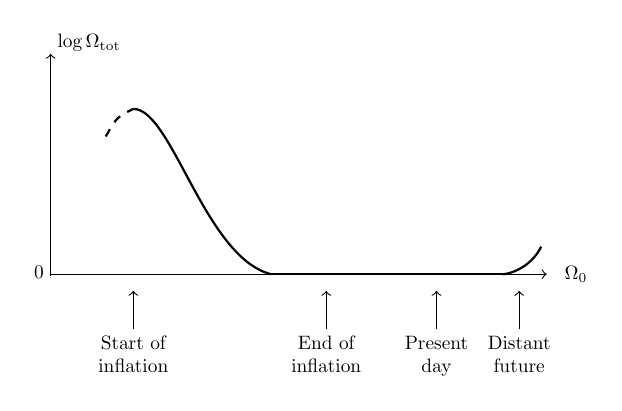
\begin{tikzpicture}[global scale = 0.7]
		\draw[->,black] (0, 0) -- (9, 0);

		\draw[black] (0, - 1pt) -- (0, + 1pt) node[anchor=east] {$0$};
		\draw[black] (9.2, 0) node[anchor=west] {$\Omega_0$};
		\draw[->,black] (0, 0) -- (0, 4);

		\draw[black] (0, 4.2) node[anchor=west] {$\log \Omega_{\text{tot}}$};
		
		\draw[->,black] (1.5, -1) -- (1.5, -0.3) node[anchor=north,align=center] at (1.5, -1) {Start of \\ inflation};
		\draw[->,black] (5, -1) -- (5, -0.3) node[anchor=north,align=center] at (5, -1) {End of \\ inflation};
		\draw[->,black] (7, -1) -- (7, -0.3) node[anchor=north, align=center] at (7, -1) {Present \\ day};
		\draw[->,black] (8.5, -1) -- (8.5, -0.3) node[anchor=north, align=center] at (8.5, -1) {Distant \\ future};
		
		\draw[thick, dashed] (1, 2.5) .. controls (1.2, 2.85) .. (1.5, 3);
		\draw[thick] (1.5, 3) .. controls (2.2, 3) and (2.8, 0.3) .. (4, 0);
		\draw[thick] (4, 0) -- (8.2, 0);
		\draw[thick] (8.2, 0) .. controls (8.3, 0) and (8.7, 0.1) .. (8.9, 0.5);
		
		
	\end{tikzpicture}
	
	\item[B. ] 视界疑难:考虑暴涨前宇宙的一个足够小的区域9,该区域小到其内部足以达到热平衡 \\
	暴涨后,这个小区域被扩大了很多倍,其尺度甚至比我们当前的可观测宇宙还要大,因此在不同方向看到的温度都一样 \\
	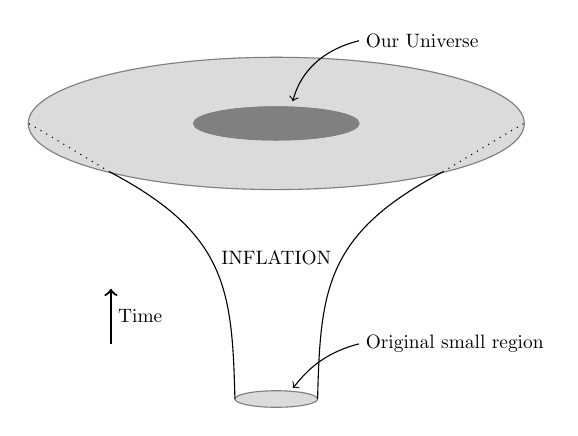
\begin{tikzpicture}[global scale = 0.7]
		\draw [fill, color=black!14!white] (0,0) ellipse [x radius=0.5*1.5cm, y radius=0.5*0.3cm];
		
		\draw [fill, color=black!14!white] (0,5) ellipse [x radius=4.5cm, y radius=1.2cm];
		\draw [fill, color=gray] (0,5) ellipse [x radius=1.5cm, y radius=0.3cm];
		
		\draw[gray] (0,0) ellipse [x radius=0.5*1.5cm, y radius=0.5*0.3cm];
		
		\draw[gray] (0,5) ellipse [x radius=4.5cm, y radius=1.2cm];
		\draw[gray] (0,5) ellipse [x radius=1.5cm, y radius=0.3cm];
		
		\draw (0.75, 0) .. controls (0.8, 2) and (0.9, 3) .. (3.02, 4.12);
		\draw (-0.75, 0) .. controls (-0.8, 2) and (-0.9, 3) .. (-3.02, 4.12);
		
		\draw[dotted] (3.02, 4.12) .. controls (4.4, 4.95) .. (4.5, 5);
		\draw[dotted] (-3.02, 4.12) .. controls (-4.4, 4.95) .. (-4.5, 5);
		
		
		\draw[black] (0, 2.8) node[anchor=north, align=center] {INFLATION};
		\draw[thick, ->,black] (-3, 1) -- (-3, 2) node[anchor=west, align=center] at (-3, 1.5) {Time};
		
		\draw[->,black] (1.5, 1) .. controls (0.7, 0.8) and (0.4, 0.3)  .. (0.3, 0.2) node[anchor=west, align=center] at (1.5, 1) {Original small region};
		
		\draw[->,black] (1.5, 6.5) .. controls (0.7, 6.3) and (0.4, 5.8)  .. (0.3, 5.4) node[anchor=west, align=center] at (1.5, 6.5) {Our Universe};
	\end{tikzpicture}
	
	\item[C. ] 重粒子残留丰度疑难:由于暴涨使得尺度因子膨胀了很多倍,这些极早期宇宙产生的重粒子的密度将被稀释到一个很小的值 \\
	但是要保证在暴涨结束后,宇宙学常数衰变的过程中不会再度产生这些“问题粒子”,这就要求暴涨结束时宇宙的温度不能太高
	
\end{itemize}

\subsubsection{对暴涨过程的估算}
\par 
以平直疑难为例,做如下五点假设:
\begin{itemize}
	\item[1. ] 暴涨终结于$10^{-34} \mathrm{s}$
	\item[2. ] 暴涨按指数膨胀方式进行
	\item[3. ] 从暴涨结束至今,宇宙是辐射主导的:$a(t) = \qty(\frac{t}{t_0})^{\frac{1}{2}}, H(t) = \frac{1}{2t}, \abs{\Omega_{\text{tot}}(t) - 1} = \frac{\abs{k}}{a^2 H^2} \propto t^{-1} \cdot t^2 \propto t$
	\item[4. ] 在暴涨开始之时$\Omega_{\text{tot}}$并非远远大于1
	\item[5. ] 假设当前时刻$\abs{\Omega_{\text{tot}} - 1} \leqslant 0.1$
\end{itemize}
\par 
辐射主导期有$\abs{\Omega_{\text{tot}}(t) - 1} \propto t$,当前宇宙的年龄约为$t_0 = 4 \times 10^{17} \mathrm{s}$,且$\abs{\Omega_{\text{tot}}(t_0) - 1} \leqslant 3 \times 10^{-53}$
\par 
在暴涨阶段$H$为常数,因此$\abs{\Omega_{\text{tot}}(t) - 1} \propto a^{-2}$,要达到暴涨结束时的值,需要尺度因子膨胀至少$10^{27}$倍
\par 
假设暴涨持续的时间为$10^{-36}$ \textasciitilde $10^{-34} \mathrm{s}$,若按照$t = H^{-1} = 10^{-36} \mathrm{s}$来估算暴涨阶段$H$的值,则$\frac{a_{\text{final}}}{a_{\text{initial}}} \simeq \ee^{H(t_{\text{final}} - t_{\text{initial}})} = \ee^{99} \simeq 10^{43}$,暴涨几乎在瞬间完成


\subsubsection{暴涨与粒子物理}
\par 
简单地引入一个宇宙学常数来描述暴涨,并假设暴涨结束后它将衰变是一种很生硬的做法,一个好的暴涨模型应该包括宇宙学常数的合理起源,和能使暴涨自然结束的方案。为了不破坏标准大爆炸理论的关于核合成等结果的预言,暴涨最晚必须在宇宙年龄为1s之前结束。大多数的暴涨模型都假设暴涨发生的时间远远早于1s,相应的能量一般很高,需要用到粒子物理学的知识

\par 
暴涨开始和结束时,宇宙的性质都将发生实质的变化,可以用相变来描述暴涨。相变一般由标量场来描述,标量场可以具有负压强,满足暴涨的条件。相变结束后,标量场可以衰变使得暴涨结束。暴涨理论是当前宇宙学研究的一个热点,大多数研究都假设暴涨由标量场描述。早期模型集中于大统一相变(强与电弱相互作用分开,$E\sim 10^{16} \mathrm{GeV}, t\sim 10^{-34} \mathrm{s}$),最近的暴涨模型主要来自超对称理论。超对称是玻色子与费米子之间的对称。超对称相变后,粒子及其伴子的性质开始不同
\end{document}